%% ============================================================
%% pynasonde — Researcher Technical Reference
%% article class with wide margins (portable, no font deps)
%%
%% Manual:
%%   cd tutorials/researcher
%%   pdflatex pynasonde_methods.tex && pdflatex pynasonde_methods.tex
%%
%% Or via project root:
%%   make tutorials
%% ============================================================
\documentclass[a4paper,11pt]{article}

% ---------- page geometry (tufte-like wide margins) ---------------
\usepackage[left=2.2cm,right=5.8cm,top=2.5cm,bottom=2.5cm,
            marginparwidth=4.8cm,marginparsep=0.5cm]{geometry}

% ---------- packages ------------------------------------------------
\usepackage{amsmath,amssymb,bm}
\usepackage{graphicx}
\usepackage{listings}
\usepackage{xcolor}
\usepackage{booktabs}
\usepackage{hyperref}
\usepackage{microtype}
\usepackage{siunitx}
\usepackage{cleveref}
\usepackage{marginnote}
\usepackage{caption}
\usepackage{multirow}
\usepackage{float}

% ---------- figure path (relative to this .tex file) ---------------
\graphicspath{{../../docs/examples/figures/}}

% ---------- margin note style ------------------------------------
\renewcommand*{\marginfont}{\footnotesize\itshape}
\newcommand{\marginnotetext}[1]{\marginnote{\footnotesize\itshape #1}}

% ---------- code style ------------------------------------------------
\definecolor{codebg}{RGB}{248,248,252}
\definecolor{codekw}{RGB}{0,0,180}
\definecolor{codestr}{RGB}{160,32,32}
\definecolor{codecom}{RGB}{0,128,0}

\lstset{
  language=Python,
  backgroundcolor=\color{codebg},
  basicstyle=\ttfamily\scriptsize,
  keywordstyle=\color{codekw}\bfseries,
  stringstyle=\color{codestr},
  commentstyle=\color{codecom}\itshape,
  showstringspaces=false,
  breaklines=true,
  frame=single,framerule=0.3pt,
  rulecolor=\color{gray!30},
  xleftmargin=4pt,xrightmargin=4pt,
  numbers=none,
}

% ---------- maths shorthands ----------------------------------------
\newcommand{\Rf}{\mathbf{R}_f}
\newcommand{\Rfinv}{\mathbf{R}_f^{-1}}
\newcommand{\avec}{\mathbf{a}}
\newcommand{\Gmat}{\mathbf{G}}
\newcommand{\wvec}{\mathbf{w}}
\newcommand{\Herm}{{}^H}
\newcommand{\tr}{\operatorname{tr}}

% ---------- title -----------------------------------------------
\title{%
  \textbf{pynasonde — Methods \& API Reference}\\[4pt]
  \large Technical guide for ionospheric researchers
}
\author{pynasonde Development Team}
\date{Version 1.0 — \today}

% =================================================================
\begin{document}
% =================================================================
\maketitle
\tableofcontents
\bigskip

\begin{abstract}
\noindent
\textbf{pynasonde} is an open-source Python toolkit for reading, analysing, and
visualising ionosonde data from both \textbf{VIPIR} and \textbf{DIGISONDE DPS4D}
instruments.  This document gives the mathematical foundations for each analysis
algorithm, the design rationale behind key implementation choices, and a compact
API cheat-sheet.  Target audience: researchers who want to understand the
algorithms, extend the toolkit, or apply it to new data sets.

\medskip\noindent
\textbf{Published reference:} Chakraborty S., Bullett T., Barjatya A., Mabie J.
(2026). pynasonde: An open-source Python library for ionosonde data processing.
\textit{SoftwareX} 34, 102617. \url{https://doi.org/10.1016/j.softx.2026.102617}
\end{abstract}

%% ==================================================================
\section{Architecture Overview}
\label{sec:architecture}
%% ==================================================================

\subsection{Published v1.0 architecture}

\marginnotetext{Figure~2 of the SoftwareX paper shows the two-module structure
(digisonde, vipir) with colour-coded data types and plotting methods.  The
analysis layer described here is entirely new post-publication.}

The library is organised into two instrument modules (\texttt{digisonde} and
\texttt{vipir}) each with dedicated parsers and plotting routines, plus a new
cross-instrument analysis layer added after publication.

\subsection{Complete file-format and class index}

\begin{table}[H]
  \centering
  \caption{All supported file formats, parser classes, and primary methods.
           \textbf{[new]} = added after SoftwareX publication.}
  \small
  \begin{tabular}{lllp{5cm}}
    \toprule
    Extension & Type & Class & Primary methods / output \\
    \midrule
    \multicolumn{4}{l}{\textit{DIGISONDE DPS4D}} \\
    \texttt{.SAO 4.3} & ASCII  & \texttt{SaoExtractor}  & \texttt{load\_SAO\_files()} with \texttt{height\_profile} or \texttt{scaled\_params} \\
    \texttt{.SAO 5.0} & XML    & \texttt{SaoExtractor}  & same API; \texttt{SaoSummaryPlots.plot\_TS()} \\
    \texttt{.RSF}     & Binary & \texttt{RsfExtractor}  & \texttt{plot\_direction\_ionogram()}, \texttt{plot\_directogram()} \textbf{[new]} \\
    \texttt{.SBF}     & Binary & \texttt{SbfExtractor}  & \texttt{extract()}, \texttt{ionogram()} \\
    \texttt{.DFT}     & ASCII  & \texttt{DftExtractor}  & \texttt{plot\_doppler\_waterfall()}, \texttt{plot\_doppler\_spectra()} \textbf{[new]} \\
    \texttt{.DVL}     & ASCII  & \texttt{DvlExtractor}  & \texttt{load\_DVL\_files()}, \texttt{plot\_dvl\_drift\_velocities()} \\
    \texttt{.SKY}     & ASCII  & \texttt{SkyExtractor}  & \texttt{extract()}, \texttt{to\_pandas()}, multi-panel \texttt{plot\_skymap()} \\
    \texttt{.EDP}     & ASCII  & \texttt{EdpExtractor}  & \texttt{extract()}, electron density profile \\
    \midrule
    \multicolumn{4}{l}{\textit{VIPIR}} \\
    \texttt{.RIQ}     & Binary & \texttt{RiqDataset}    & \texttt{create\_from\_file()}, SCT + PCT, \texttt{VIPIR\_VERSION\_MAP} \\
    \texttt{.RIQ}     & —      & \texttt{EchoExtractor} \textbf{[new]} & 7-param Dynasonde echoes (h, A, V*, EP, PP, XL, YL) \\
    \texttt{.RIQ}     & —      & \texttt{IonogramFilter} \textbf{[new]} & 6-stage filter: RFI, EP, multi-hop, DBSCAN, RANSAC, temporal \\
    \texttt{.NGI}     & NetCDF & \texttt{DataSource}    & \texttt{load()}, multi-file data cube aggregation \\
    \texttt{.NGI}     & —      & \texttt{AutoScaler}    & noise profiling, segmentation, binary trace extraction \\
    \midrule
    \multicolumn{4}{l}{\textit{Analysis layer (all new post-v1.0)}} \\
    —  & — & \texttt{PolarizationClassifier} & O/X mode separation via PP; hemisphere-aware \\
    —  & — & \texttt{TrueHeightInversion}    & Titheridge/POLAN lamination; \texttt{EDPResult} \\
    —  & — & \texttt{AbsorptionAnalyzer}     & LOF, O/X differential, calibrated, $\kappa(z)$ \\
    —  & — & \texttt{SpreadFAnalyzer}        & Range / frequency / mixed spread-F classification \\
    —  & — & \texttt{IrregularityAnalyzer}   & EP structure function $\to$ $\alpha(h)$, outer scale, anisotropy \\
    —  & — & \texttt{IonogramScaler}         & foF2, foE, $h'$F, MUF from O-mode trace \\
    —  & — & \texttt{EsCaponImager}          & Capon cross-spectrum, $\Delta r = r_0/K$ \\
    —  & — & \texttt{RiqAggregator}          & Multi-file A+B+C, $\sim$24~dB SNR gain \\
    —  & — & \texttt{NeXtYZInverter}         & WSI model + Hamiltonian ray-tracing, 3-D $N(h,x,y)$ \\
    —  & — & \texttt{FullPipeline}           & End-to-end RIQ $\to$ N(h) automation \\
    \bottomrule
  \end{tabular}
\end{table}

%% ==================================================================
\section{Instrument Overview}
\label{sec:instruments}
%% ==================================================================

\subsection{VIPIR}

VIPIR (Vertical Incidence Pulsed Ionospheric Radar) records raw in-phase and
quadrature (IQ) samples in binary \texttt{.RIQ} files.  Each file contains a
Sounding Control Table (SCT) followed by one Pulse Configuration Table (PCT)
record per transmitted pulse.  The IQ cube for one sounding frequency has shape
$(\text{pulse\_count}, \text{gate\_count}, \text{rx\_count})$.

\marginnotetext{WI937 (Wallops Island): 4 pulses/freq, 960 gates ($r_0=1.499$~km),
8 Rx channels.  PL407 (Prudhoe Bay): newer format, data\_type=2.}

\begin{lstlisting}[caption={VIPIR — load a RIQ file}]
from pynasonde.vipir.riq.parsers.read_riq import RiqDataset, VIPIR_VERSION_MAP

riq = RiqDataset.create_from_file(
    "data/WI937_20220821.RIQ",
    vipir_config=VIPIR_VERSION_MAP.configs[1],  # data_type=1 (older format)
)
sct = riq.sct    # SoundingControlTable
# Key fields: sct.timing.gate_count, sct.timing.gate_step (us),
#             sct.station.rx_count, sct.station.rx_position
\end{lstlisting}

\subsection{DIGISONDE DPS4D}

The Digisonde DPS4D family stores data in several formats:

\marginnotetext{SAO is the primary product for most science applications.
RSF/SBF give access to raw amplitude and phase.  DFT contains the full
Doppler spectrum per height.}

\begin{center}
\begin{tabular}{llp{6cm}}
  \toprule
  Extension & Class & Contents \\
  \midrule
  \texttt{.SAO}  & \texttt{SaoExtractor}  & Scaled parameters (foF2, hmF2, MUF) + N(h) profile \\
  \texttt{.RSF}  & \texttt{RsfExtractor}  & Raw amplitude + phase per frequency/height/azimuth \\
  \texttt{.SBF}  & \texttt{SbfExtractor}  & Binary raw sounding (alternative to RSF) \\
  \texttt{.DFT}  & \texttt{DftExtractor}  & Per-height Doppler spectra (velocity vs.\ height) \\
  \texttt{.DVL}  & \texttt{DvlExtractor}  & Drift velocity estimates (Vx, Vy, Vz) \\
  \texttt{.SKY}  & \texttt{SkyExtractor}  & Sky map (polar arrival-direction map) \\
  \bottomrule
\end{tabular}
\end{center}

\begin{lstlisting}[caption={DIGISONDE — load SAO files in parallel}]
from pynasonde.digisonde.parsers.sao import SaoExtractor

df = SaoExtractor.load_SAO_files(
    folders=["data/KR835/"],
    func_name="height_profile",   # or "scaled_params"
    n_procs=4,
)
# df columns: datetime, height_km, plasma_freq_mhz, electron_density_cm3, ...
\end{lstlisting}

\begin{figure}[H]
  \centering
  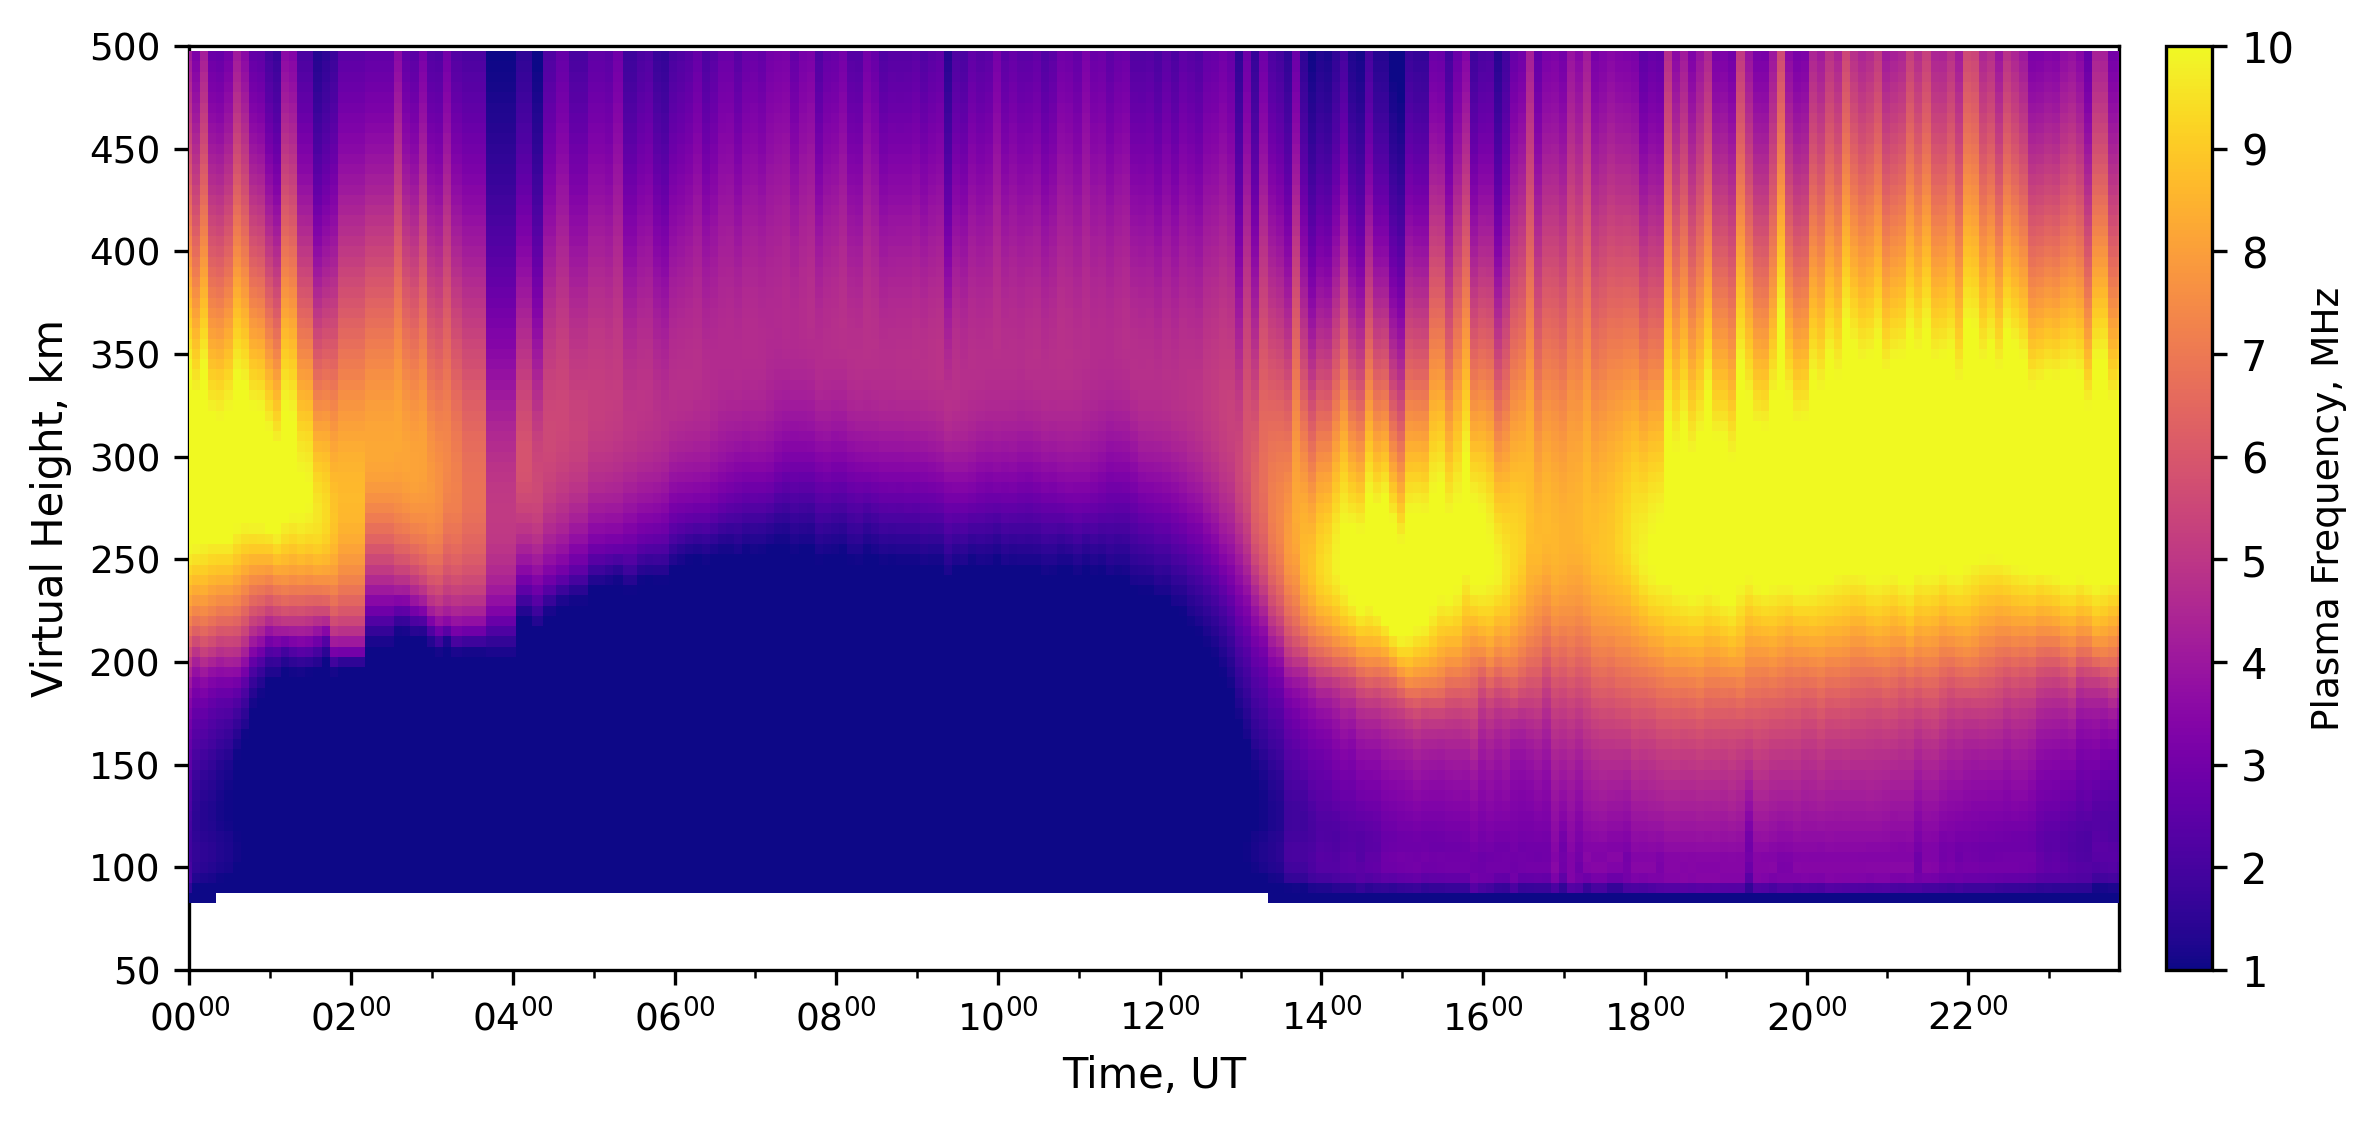
\includegraphics[width=0.90\linewidth]{sao_isodensity_KR835.png}
  \caption{Daily isodensity contour from DPS4D SAO files at KR835.
           Each column is one N(h) profile; colour encodes electron density
           ($\text{cm}^{-3}$, log scale).}
  \label{fig:sao_isodensity}
\end{figure}

\begin{figure}[H]
  \centering
  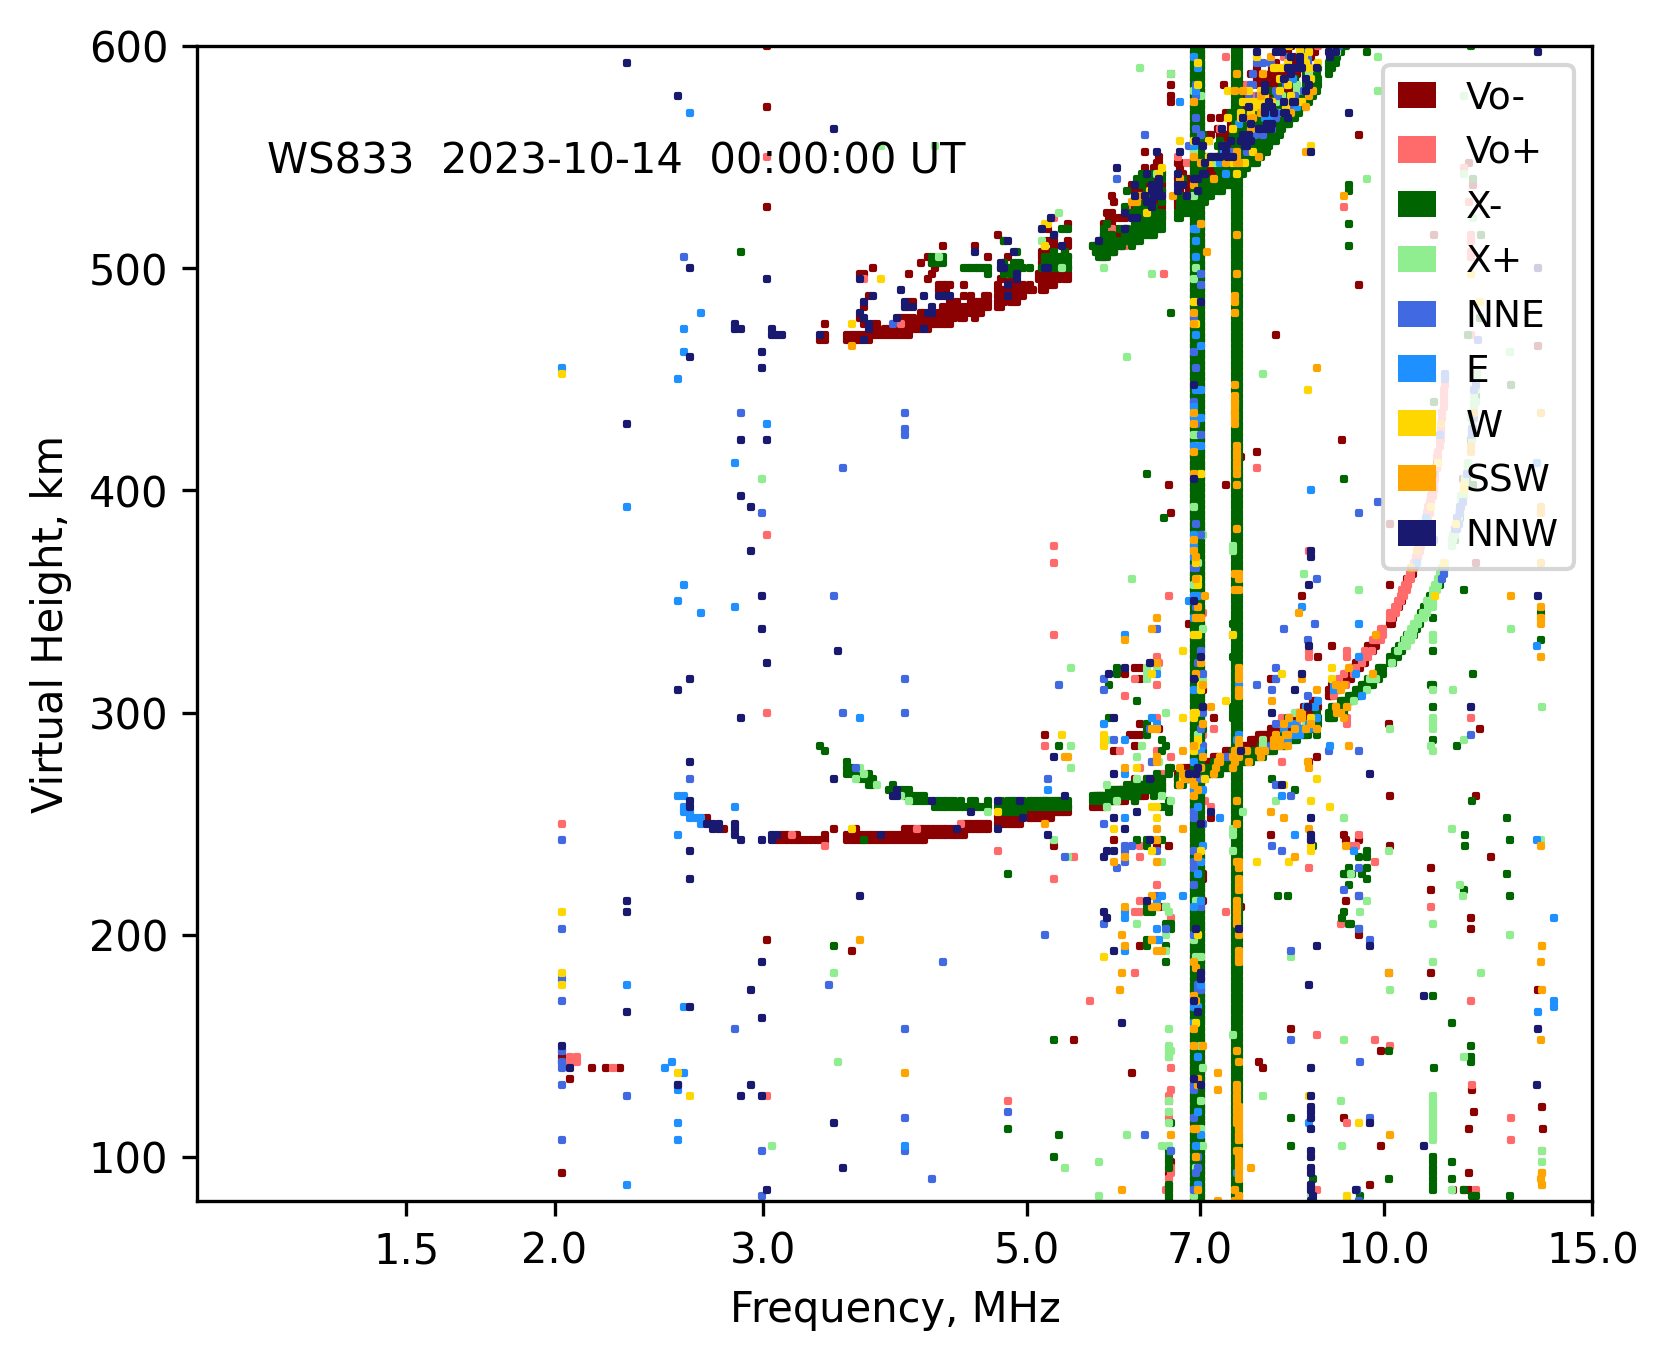
\includegraphics[width=0.90\linewidth]{rsf_direction_ionogram_KR835.png}
  \caption{Direction-coded ionogram from a DPS4D RSF sounding at KR835.
           Colour encodes the echo arrival azimuth.}
  \label{fig:rsf_ionogram}
\end{figure}

\begin{figure}[H]
  \centering
  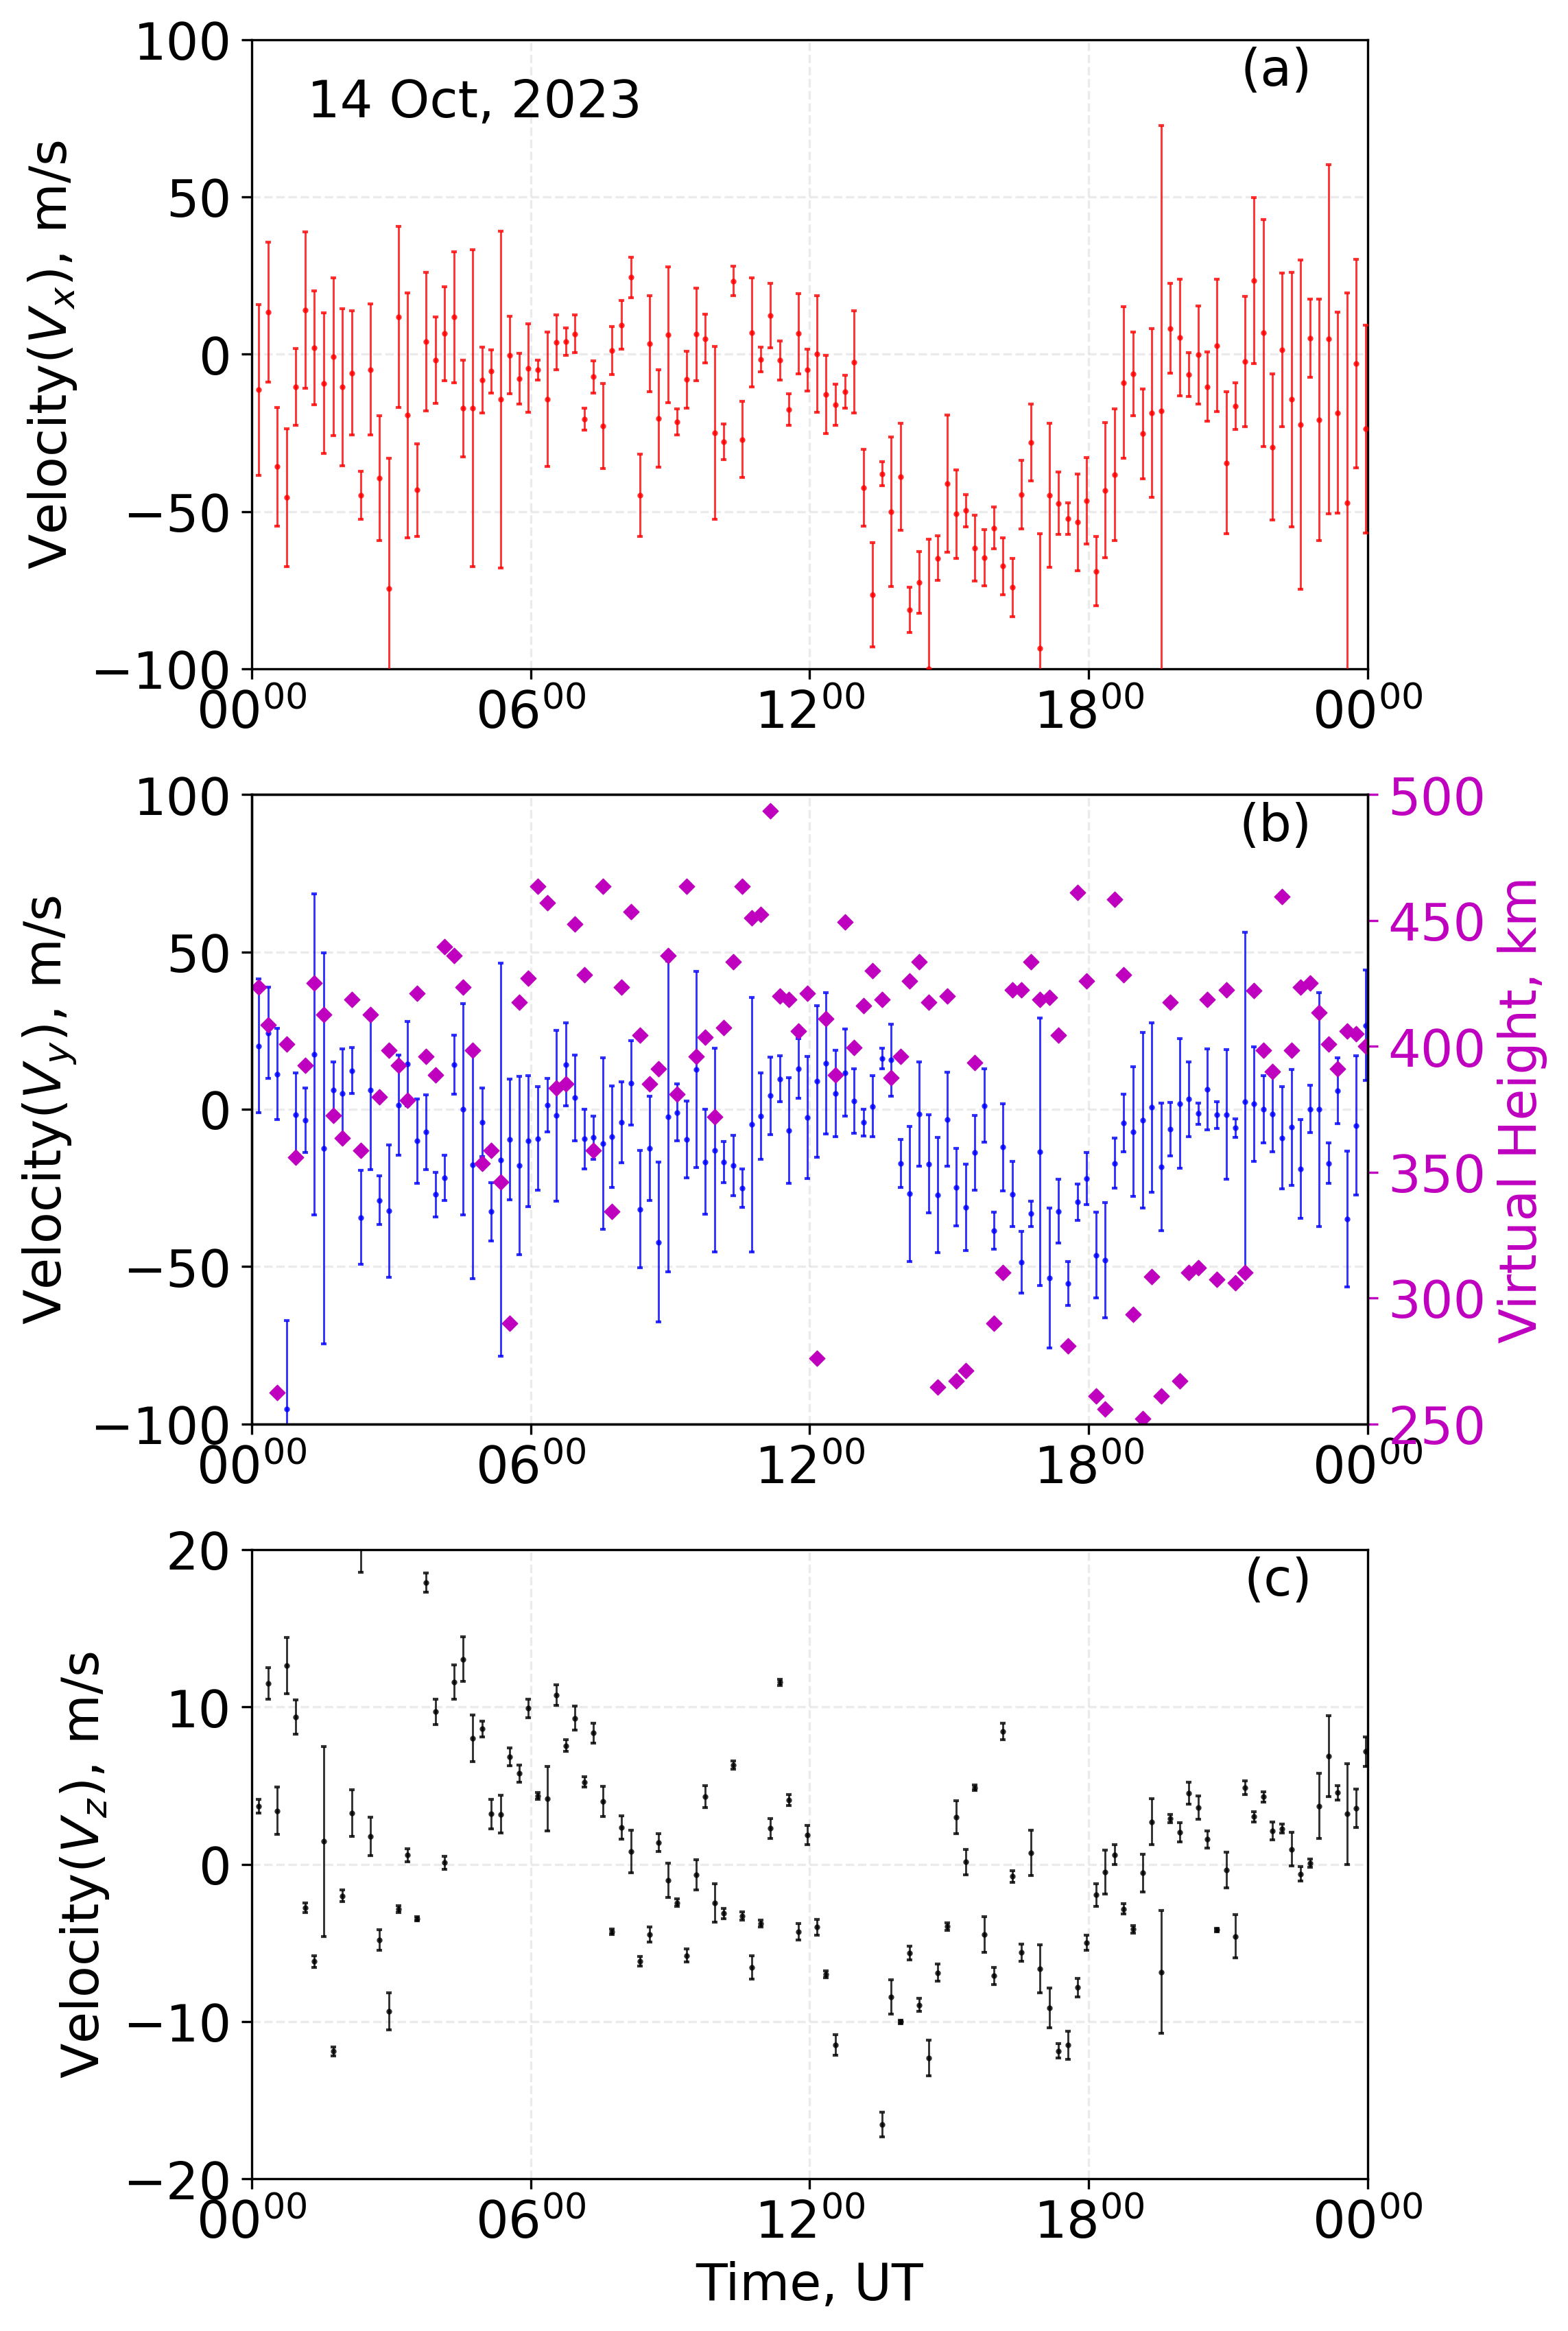
\includegraphics[width=0.90\linewidth]{stackplots_dvl.png}
  \caption{Three-panel drift velocity stack plot from DPS4D DVL files.
           Panels: $V_x$ (east), $V_y$ (north), $V_z$ (vertical), with
           virtual-height overlay.}
  \label{fig:dvl_stack}
\end{figure}

%% ==================================================================
\section{VIPIR Echo Extraction \& Filtering}
\label{sec:echo}
%% ==================================================================

\subsection{Seven-parameter echo extraction}

\texttt{EchoExtractor} computes the seven Dynasonde-style echo parameters —
height, amplitude, Doppler velocity V*, wavefront residual EP, polarization
chirality PP, and direction cosines XL/YL — from the pulse-compressed IQ cube.

\begin{figure}[H]
  \centering
  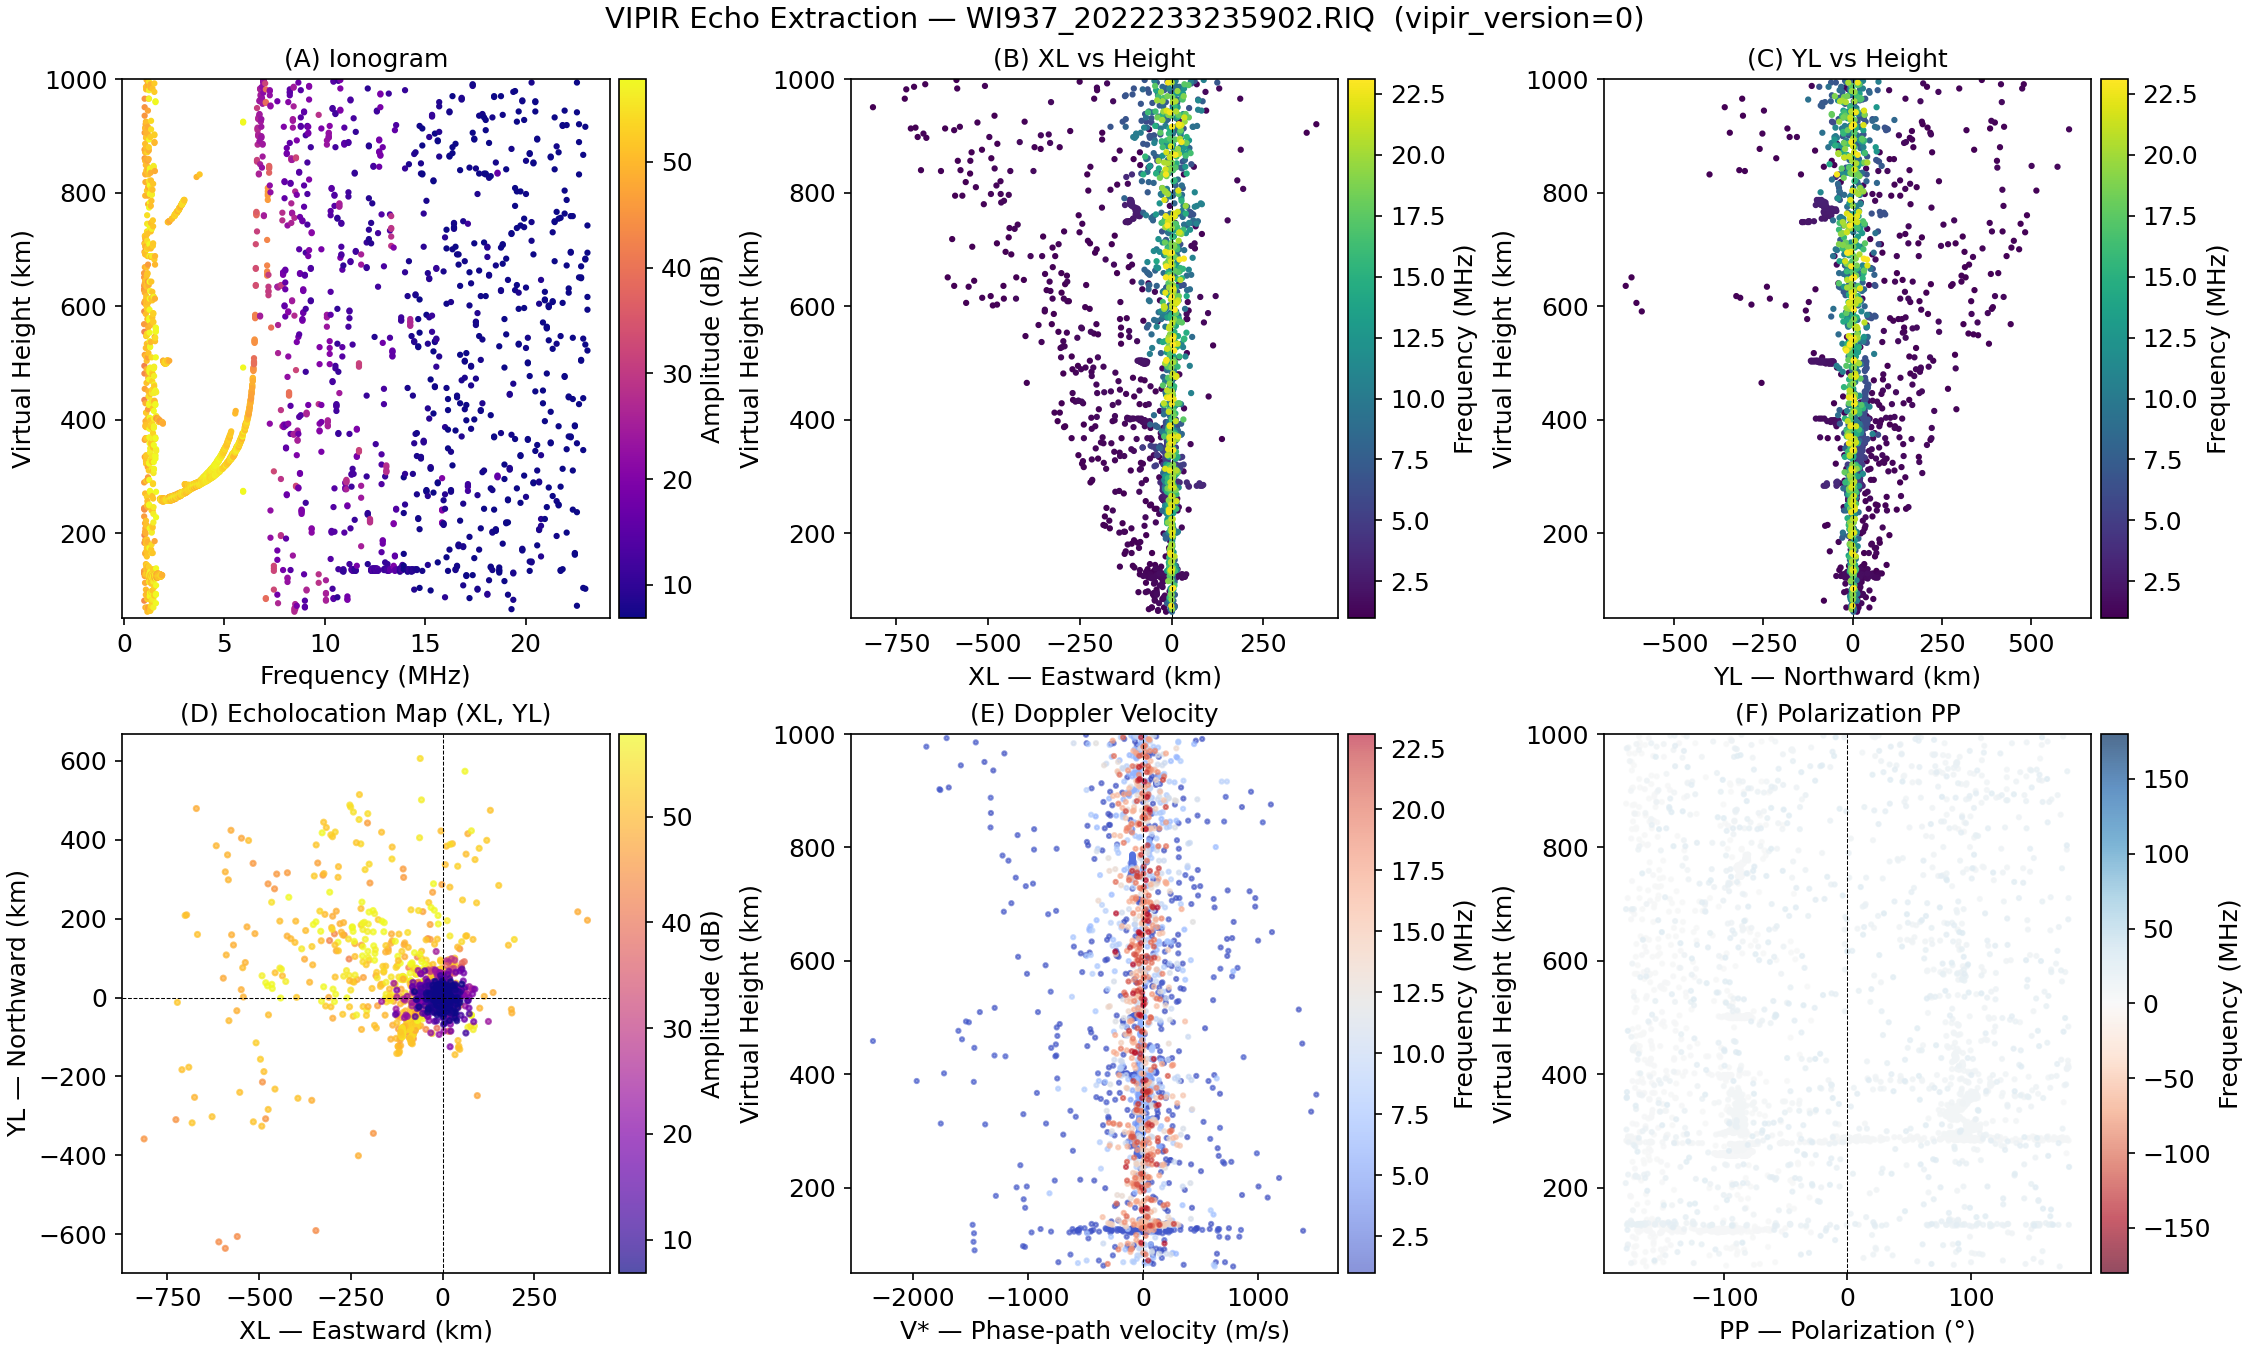
\includegraphics[width=0.90\linewidth]{echo_extraction_wi937.png}
  \caption{Six-panel diagnostic for WI937 echo extraction: ionogram (A),
           XL (B), YL (C), echo location map (D), Doppler V* (E), PP (F).}
  \label{fig:echo_wi937}
\end{figure}

\begin{lstlisting}[caption={Echo extraction and filtering}]
from pynasonde.vipir.riq.echo import EchoExtractor
from pynasonde.vipir.riq.parsers.filter import IonogramFilter

extractor = EchoExtractor(sct=riq.sct, pulsets=riq.pulsets,
                          snr_threshold_db=3.0).extract()
df = extractor.to_dataframe()

filtered = IonogramFilter(snr_threshold_db=6.0, ep_threshold_deg=30.0,
                          use_dbscan=True, use_ransac=True).fit(df)
\end{lstlisting}

%% ==================================================================
\section{Capon Cross-Spectrum Es Layer Imaging}
\label{sec:capon}
%% ==================================================================

\subsection{Physical motivation}

Sporadic-E (Es) layers are thin metallic-ion sheets at 90--130~km altitude.
Their vertical thickness ($< 1$~km) is below the native range resolution of
most ionosondes ($r_0 = 1.5$--$4$~km).

\marginnotetext{Liu et al.\ (2023) demonstrated 384~m resolution from a 3.84~km
native gate using 256 pulses from the WISS digisonde.}

The pulse-compressed range profile $R_{ss}(t)$ is a complex sequence of $V$
samples.  Its FFT (the \emph{cross-power spectrum}) is
\begin{equation}
  G_{ss}(f_m) = \operatorname{FFT}\{R_{ss}\}(f_m)
              = U(f_m)\,e^{j4\pi r f_m/c},
  \label{eq:Gss}
\end{equation}
where $U(f)=|S(f)|^2$ encodes signal power and the exponential encodes range $r$.

\subsection{Hankel subband matrix and covariance}

Partition $G_{ss}$ into a Hankel matrix $\Gmat$ of shape $(Z,\,V-Z+1)$:
\begin{equation}
  G[i,j] = G_{ss}[f_{i+j}],\quad i=0\ldots Z-1,\; j=0\ldots V-Z.
  \label{eq:hankel}
\end{equation}
The spatial covariance with diagonal loading $\varepsilon$:
\begin{equation}
  \Rf = \frac{\Gmat\Gmat\Herm}{V-Z+1}
        + \varepsilon\,\frac{\tr(\Rf)}{Z}\,\mathbf{I}_Z.
  \label{eq:Rf}
\end{equation}

\subsection{Capon pseudospectrum}

Steering vector $\avec(\omega_\ell)\in\mathbb{C}^Z$ with
$a_k(\omega_\ell) = e^{jk\omega_\ell}$ and $\omega_\ell = 2\pi\ell/(KV)$:
\begin{equation}
  \boxed{P\!\left(\frac{\ell r_0}{K}\right)
    = \frac{1}{\avec\Herm(\omega_\ell)\,\Rfinv\,\avec(\omega_\ell)}},
  \quad \ell = 1,\ldots,KV.
  \label{eq:capon}
\end{equation}
Effective range resolution: $\Delta r = r_0/K$.

\subsection{Singularity constraints}
\label{sec:singularity}

\marginnote{\footnotesize\textit{Parameter roles:}\\[2pt]
  \begin{tabular}{@{}lp{3cm}@{}}
    $Z$ & Covariance size; affects rank of $\Rf$ \\
    $K$ & Output grid only; does \textbf{not} enter $\Rf$ \\
  \end{tabular}}

$\Rf$ has shape $(Z,Z)$ and rank at most $V-Z+1$.  For full rank:
\begin{equation}
  V - Z + 1 \ge Z \quad\Longrightarrow\quad Z \le \frac{V+1}{2}.
  \label{eq:Zconstraint}
\end{equation}
\textbf{$K$ has no singularity constraint.}  Earlier implementations
incorrectly clipped $K \le \lfloor V/Z\rfloor$; pynasonde $\ge$1.0 removes
this constraint entirely.

\marginnotetext{Liu et al.\ Fig.~1: $Z=50$ (unresolved), $Z=100$ (resolved,
  optimal), $Z=150$ ($>(V{+}1)/2$, rank-deficient, partially recovered via
  diagonal loading).}

\begin{figure}[H]
  \centering
  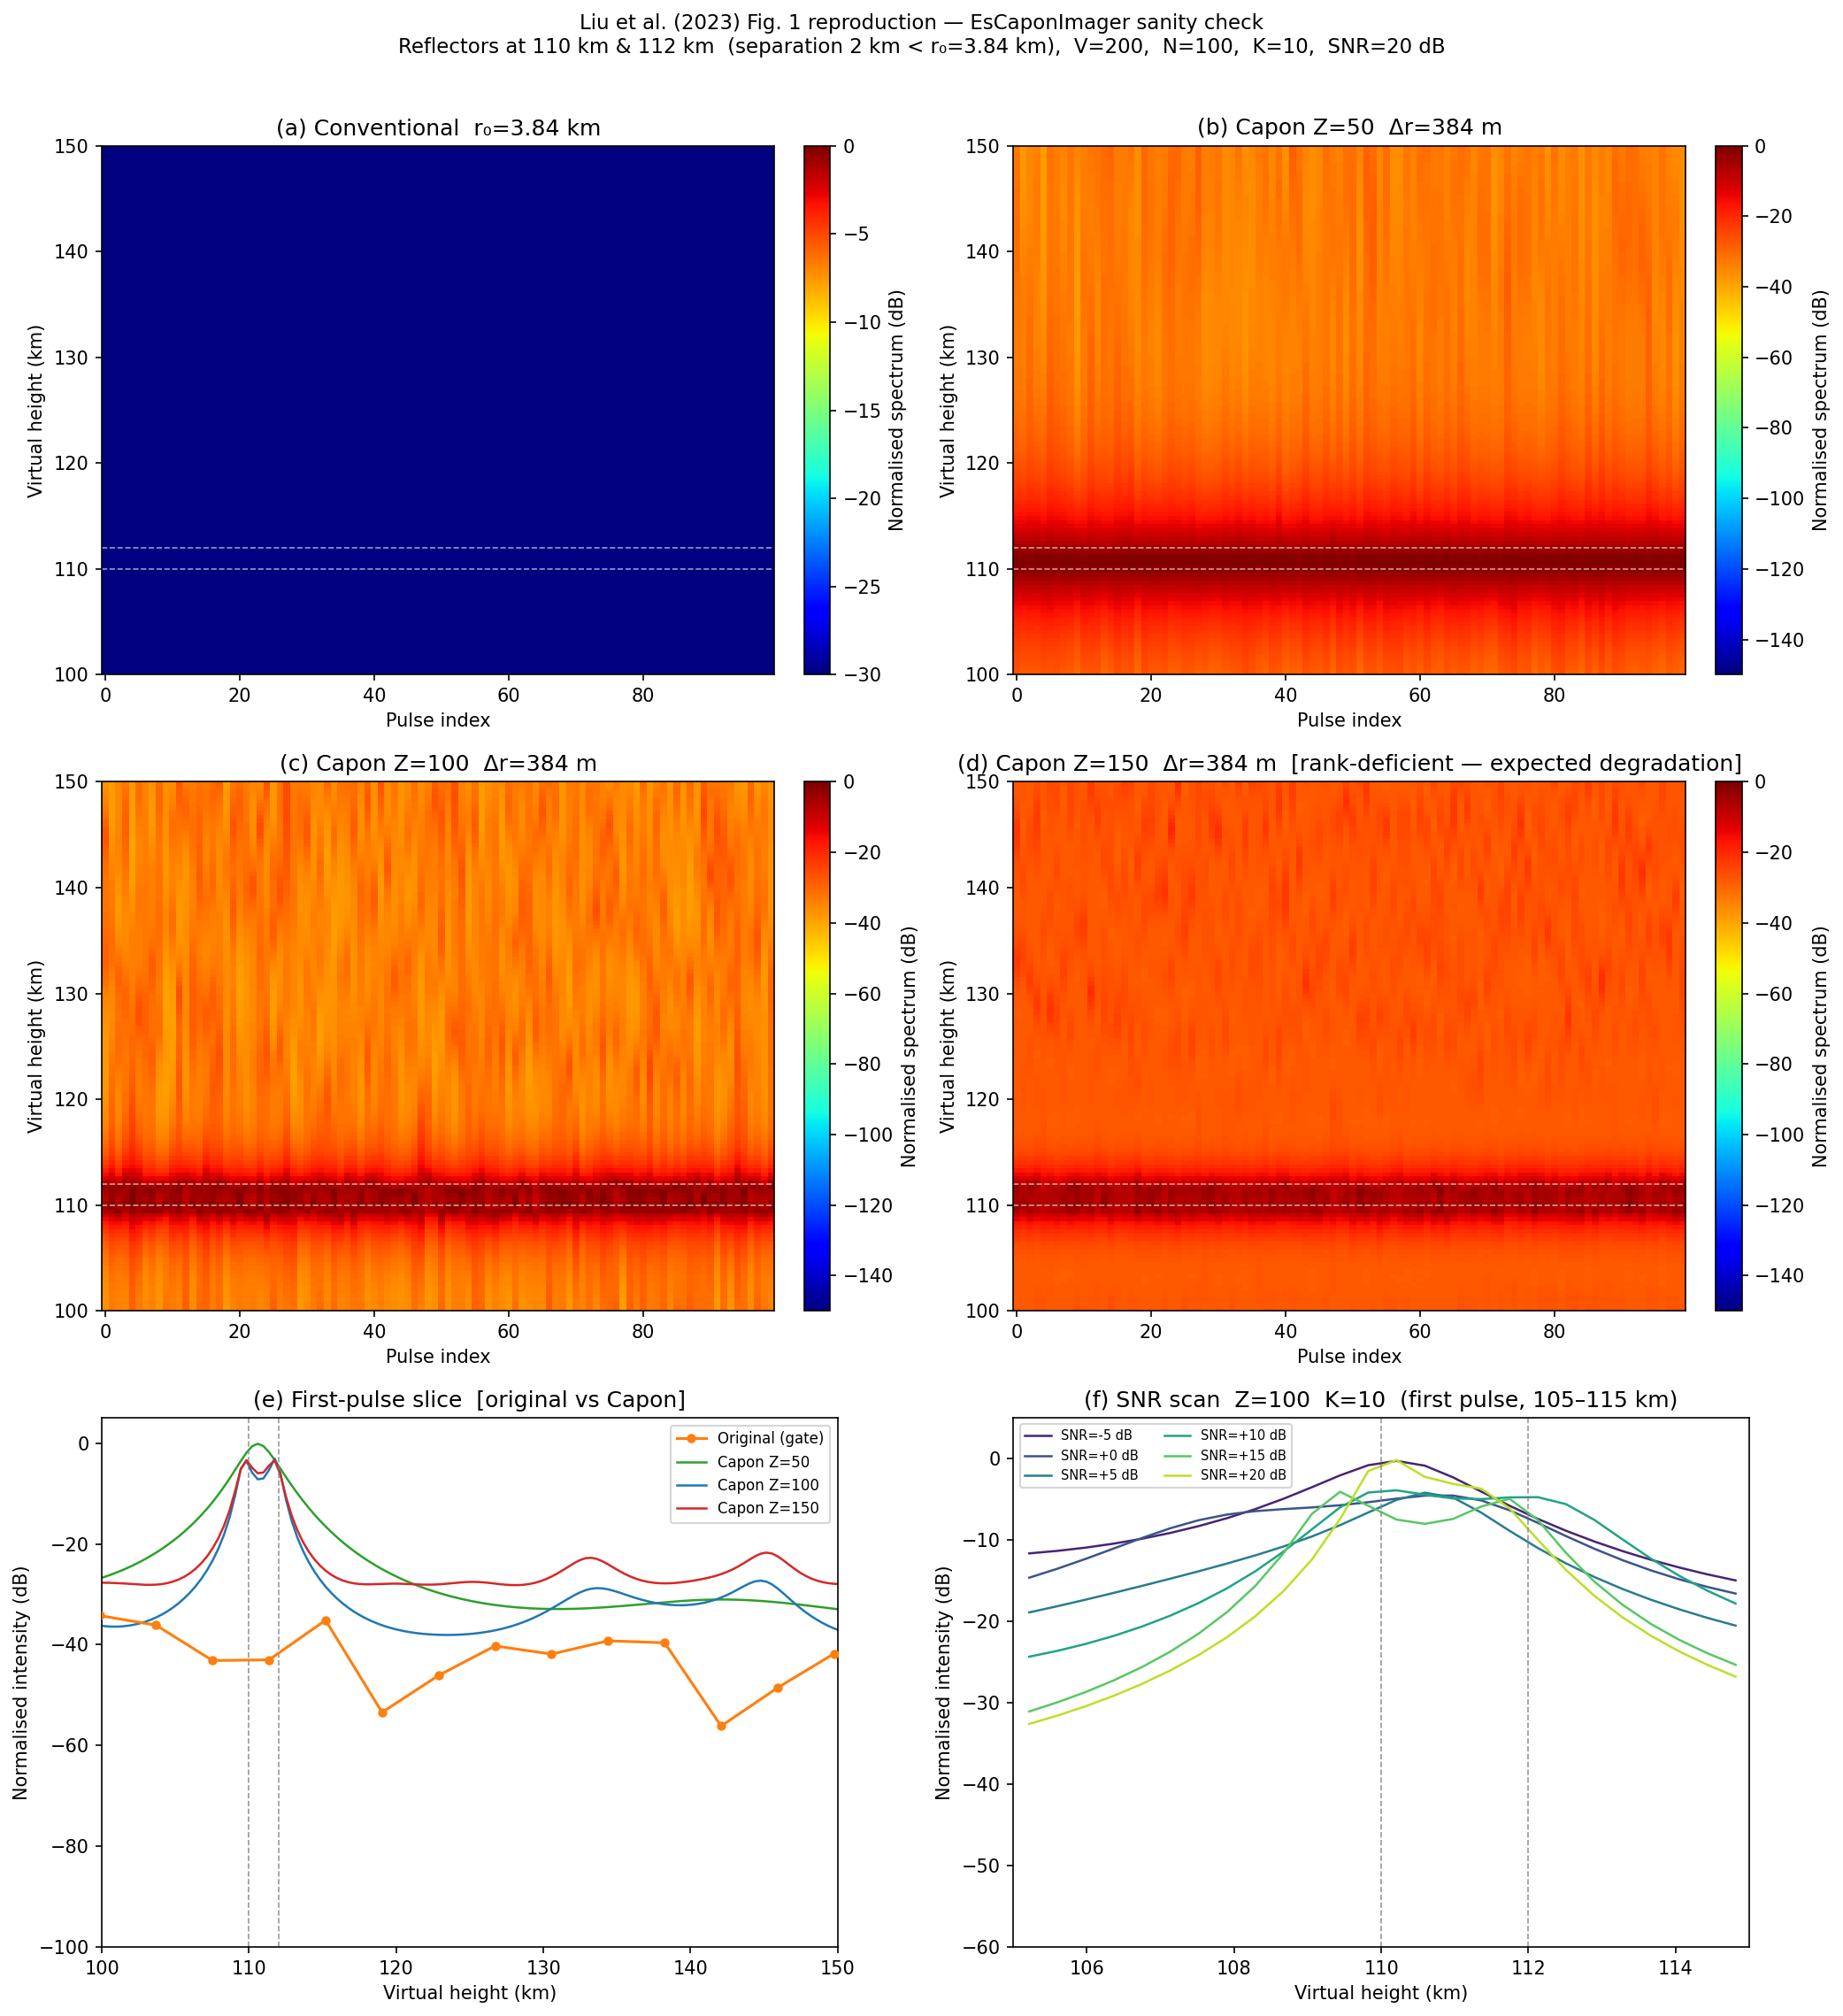
\includegraphics[width=0.90\linewidth]{es_imaging_sanity_check.png}
  \caption{Synthetic sanity check reproducing Liu et al.\ (2023) Fig.~1.
           Two layers at 110 and 112~km ($r_0=3.84$~km, $V=200$, $K=10$).
           (a)~Conventional; (b)~$Z=50$; (c)~$Z=100$; (d)~$Z=150$; (e)~first pulse; (f)~SNR scan.}
  \label{fig:sanity}
\end{figure}

\begin{figure}[H]
  \centering
  \begin{minipage}{0.48\linewidth}
    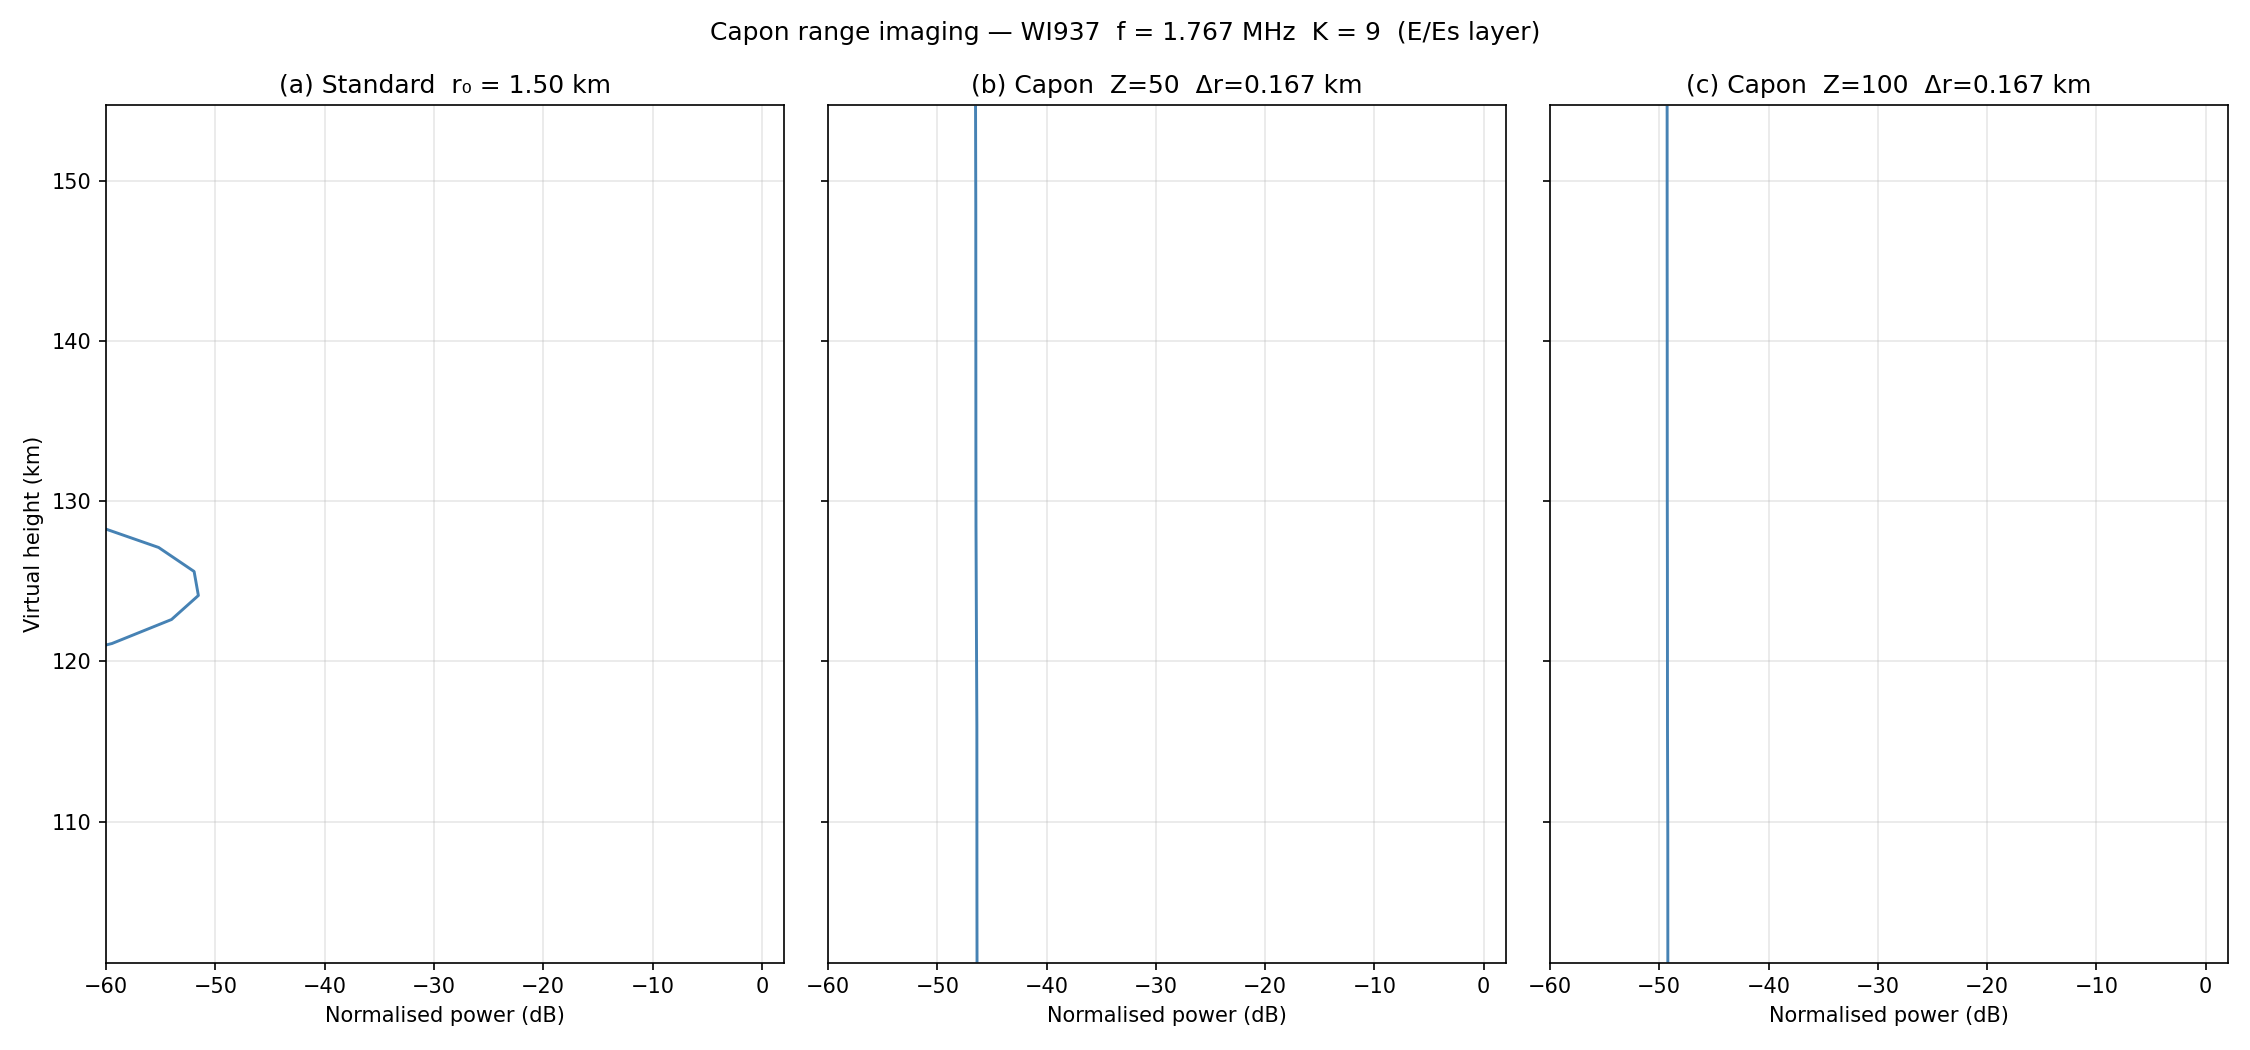
\includegraphics[width=\linewidth]{analysis_es_imaging.png}
    \caption{Single-file Es Capon image (1-D profile).}
    \label{fig:es_single}
  \end{minipage}\hfill
  \begin{minipage}{0.48\linewidth}
    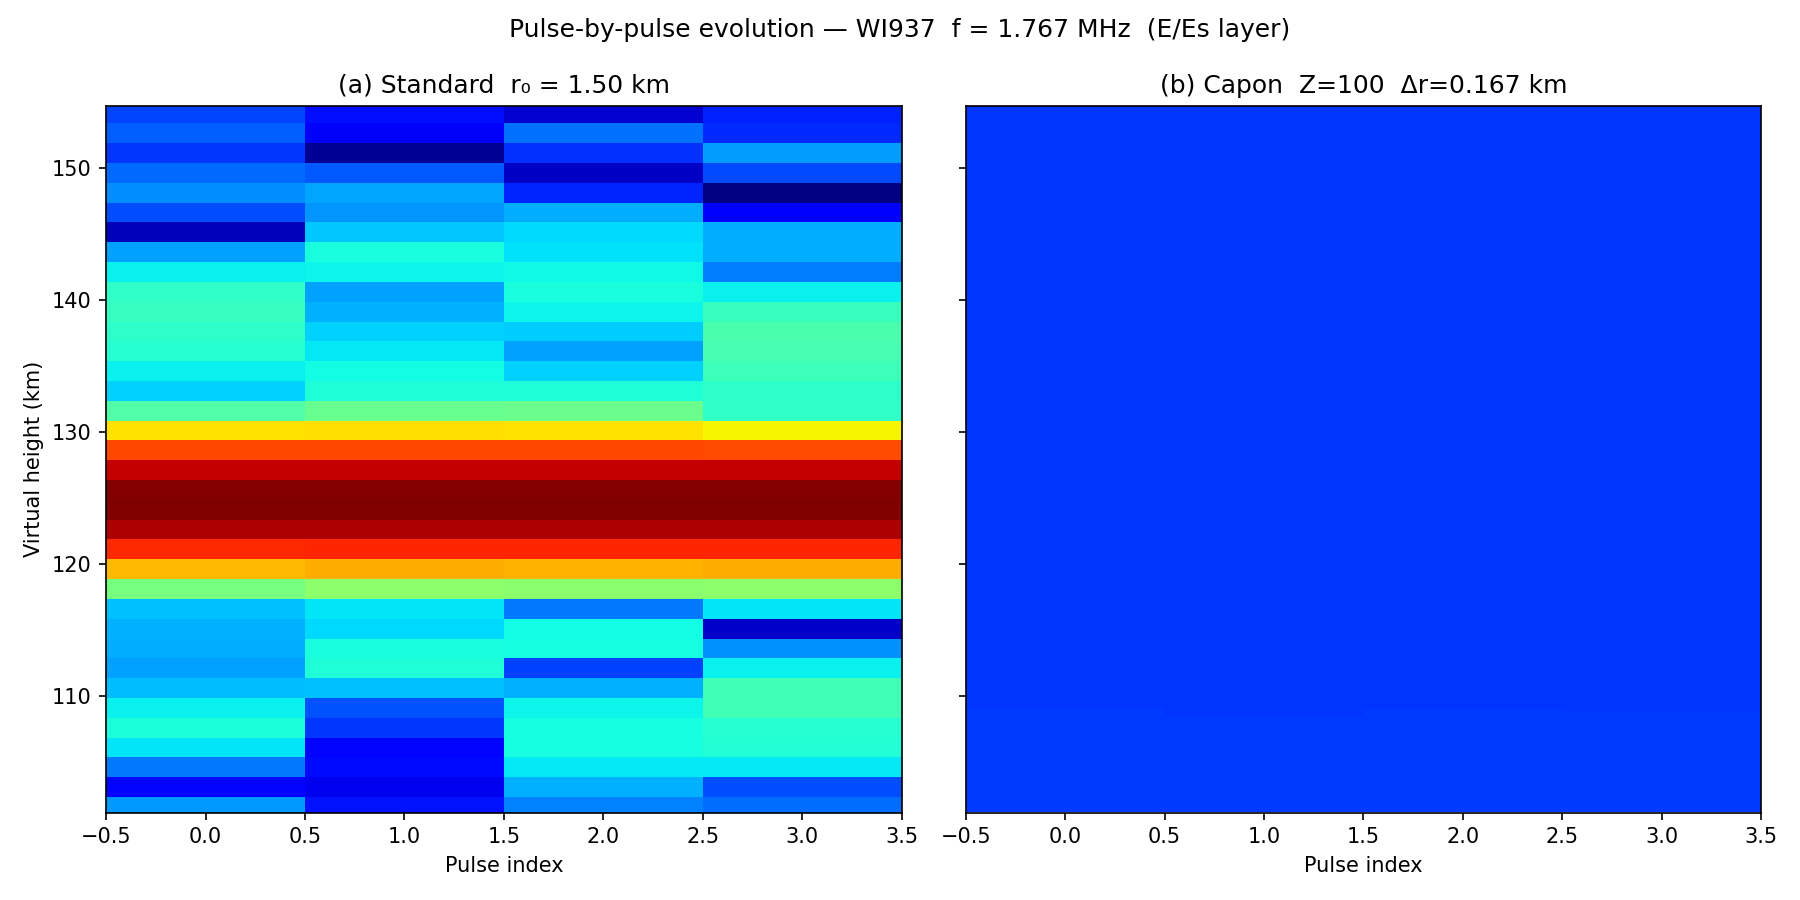
\includegraphics[width=\linewidth]{analysis_es_imaging_rti.png}
    \caption{Slow RTI from \texttt{RiqAggregator} (A+B+C, 8 files).}
    \label{fig:es_rti}
  \end{minipage}
\end{figure}

\begin{lstlisting}[caption={EsCaponImager — single file}]
from pynasonde.vipir.analysis import EsCaponImager
imager = EsCaponImager(n_subbands=100, resolution_factor=10,
                       gate_spacing_km=1.499, gate_start_km=90.0)
result = imager.fit(iq_cube)
\end{lstlisting}

%% ==================================================================
\section{Multi-File A+B+C Combining (RiqAggregator)}
\label{sec:aggregator}
%% ==================================================================

\subsection{Combining strategy}

\marginnotetext{Calibrated Rx weights from the antenna position table
(SCT header \texttt{station.rx\_position}) will be supported once the RIQ
header reader exposes them.}

\textbf{Option A} — Coherent Rx beamforming:
\begin{equation}
  R_{\mathrm{beam}}[p,g] = \mathbf{S}[p,g,:]\,\wvec^*, \quad
  \Delta\mathrm{SNR} = 10\log_{10}(n_{rx})\;\mathrm{dB}.
\end{equation}
\textbf{Option B} — Incoherent pulse averaging (per file):
\begin{equation}
  P_{\mathrm{file}} = \frac{1}{n_p}\sum_{p} P_{\mathrm{Capon}}(R_{\mathrm{beam}}[p,:]).
\end{equation}
\textbf{Option C} — Incoherent file stacking:
\begin{equation}
  P_{\mathrm{final}} = \frac{1}{n_f}\sum_{f} P_{\mathrm{file},f}.
\end{equation}

\marginnote{\footnotesize\textit{SNR budget} (8 files $\times$ 4 pulses $\times$ 8 Rx):\\[2pt]
  \begin{tabular}{@{}lc@{}}
    \toprule Step & Gain \\ \midrule
    Opt.\ A (8 Rx) & $+9$~dB \\
    Opt.\ B (4p avg) & $\div 4$ var \\
    Opt.\ C (8f stack) & $\div 8$ var \\ \midrule
    \textbf{Total} & $\approx +24$~dB \\ \bottomrule
  \end{tabular}}

\begin{lstlisting}[caption={RiqAggregator — multi-file A+B+C}]
from pynasonde.vipir.analysis import RiqAggregator
agg = RiqAggregator(n_subbands=100, resolution_factor=10,
                    output_mode="slow_rti")  # or "single"
result = agg.fit(file_list, freq_target_khz=5000.0, freq_tol_khz=50.0)
\end{lstlisting}

%% ==================================================================
\section{HF Radio Absorption}
\label{sec:absorption}
%% ==================================================================

No-field, weak-collision Appleton-Hartree absorption rate (dB~km$^{-1}$):
\begin{equation}
  \kappa(h) = \frac{4.343\,\nu(h)\,X(h)}{c_{\mathrm{km}}\sqrt{1-X(h)}},
  \qquad X = (f_p/f)^2.
  \label{eq:kappa}
\end{equation}
LOF index: $A = f_{\min}^2 - f_{\mathrm{ref}}^2\;[\mathrm{MHz}^2]$.
Differential O/X: $\Delta L(f) = \mathrm{SNR}_O - \mathrm{SNR}_X\;[\mathrm{dB}]$.

\begin{figure}[H]
  \centering
  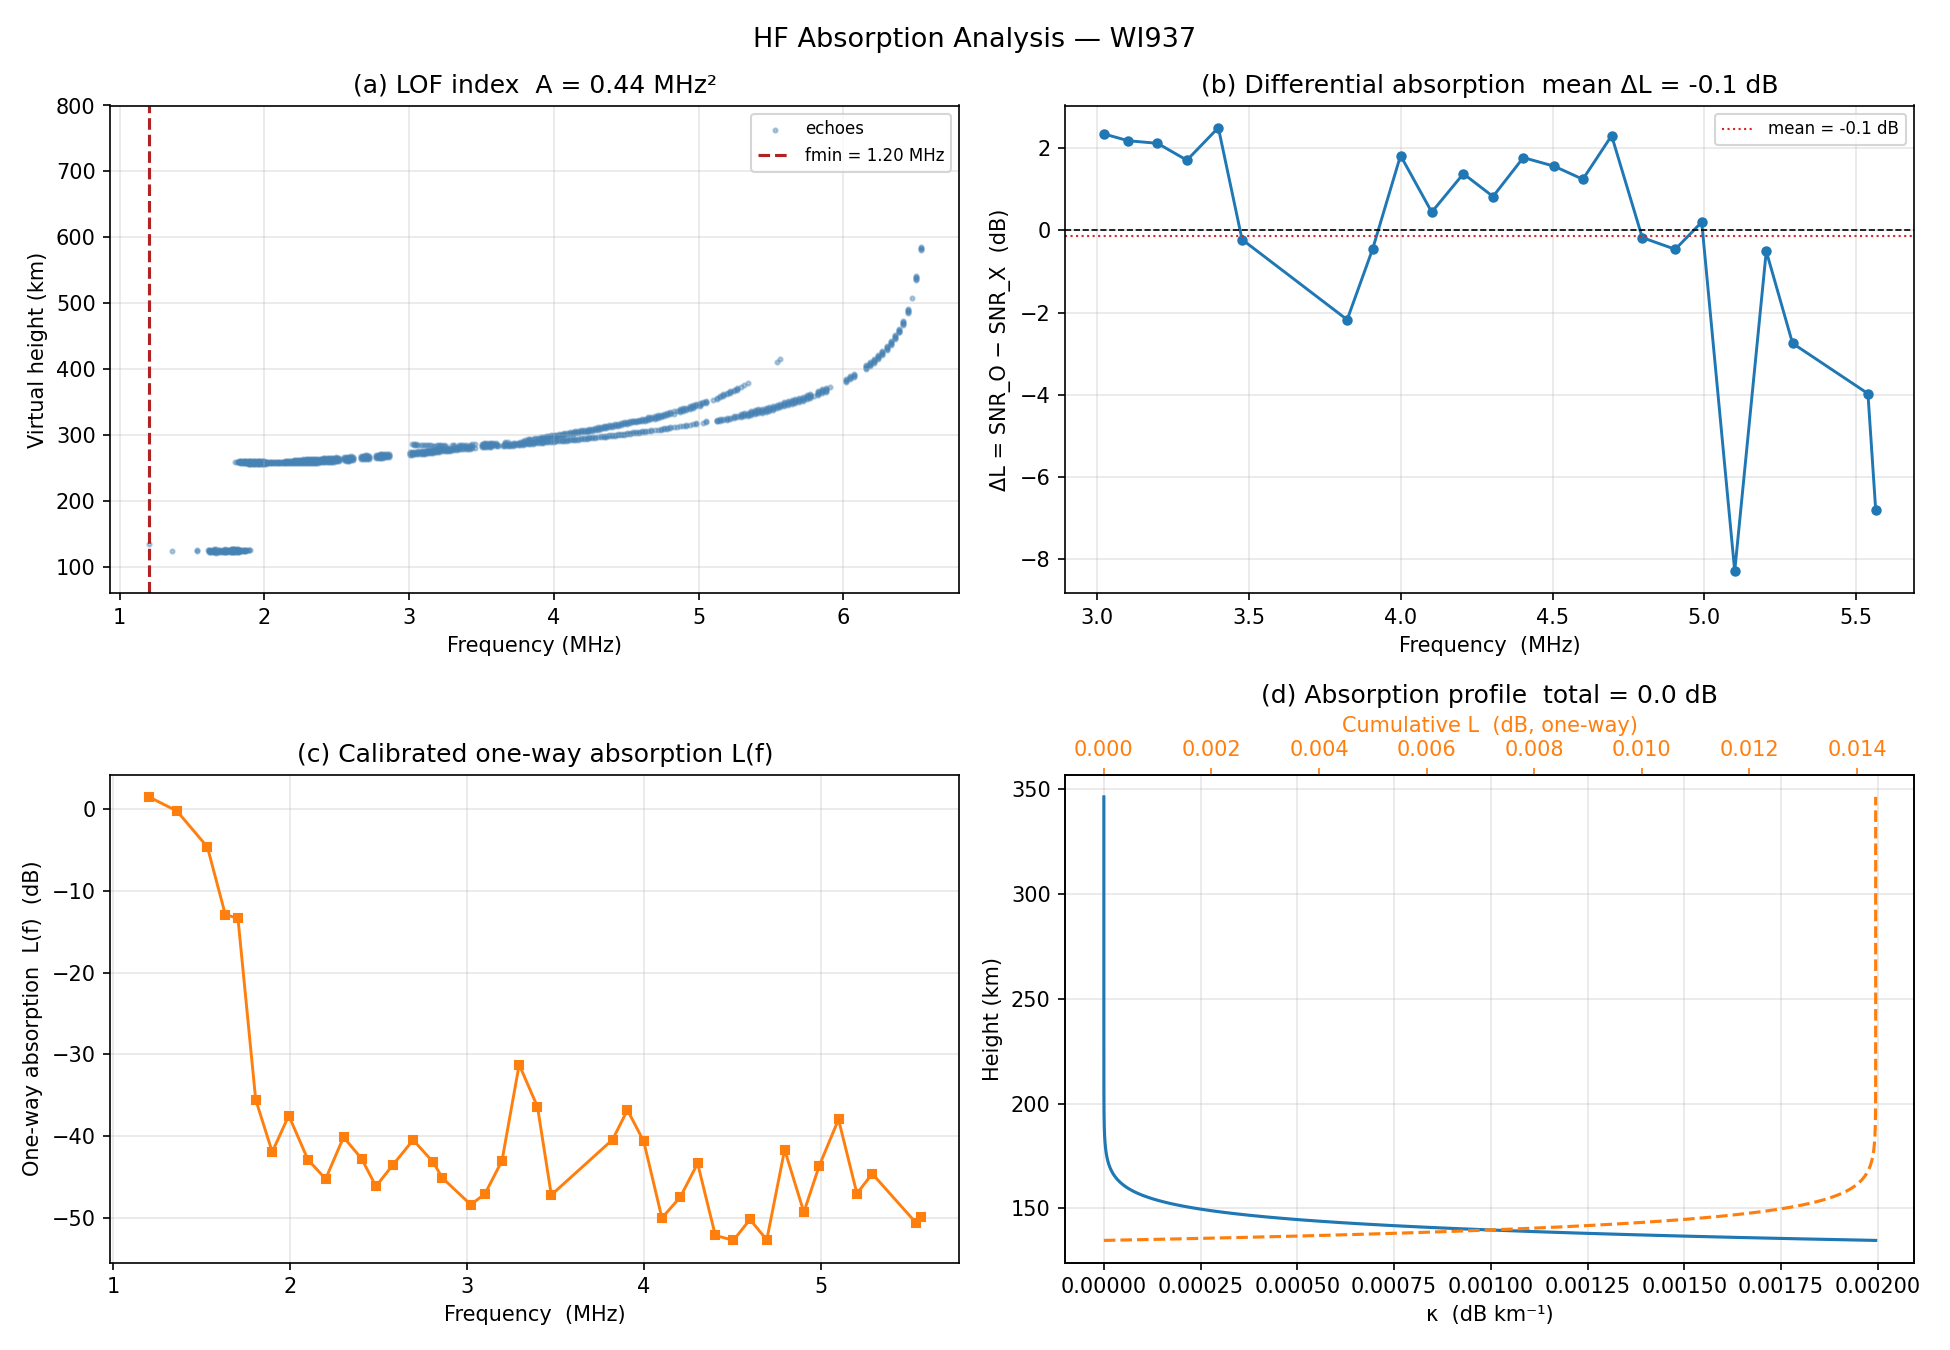
\includegraphics[width=0.90\linewidth]{analysis_absorption.png}
  \caption{Absorption analysis panels: (a)~LOF index, (b)~differential O/X
           $\Delta L(f)$, (c)~total calibrated $L(f)$, (d)~height-resolved $\kappa(z)$.}
  \label{fig:absorption}
\end{figure}

\begin{lstlisting}[caption={AbsorptionAnalyzer — all four estimators}]
from pynasonde.vipir.analysis import AbsorptionAnalyzer
import numpy as np

aa = AbsorptionAnalyzer(f_ref_mhz=1.0)
lof  = aa.lof_absorption(filtered_df)                           # LOF
diff = aa.differential_absorption(pol.annotated_df)             # O/X
total= aa.total_absorption(filtered_df, tx_eirp_dbw=70.0)       # calibrated
prof = aa.absorption_profile(edp, nu_hz=lambda h: 1e6*np.exp(-h/8.0))  # k(z)
\end{lstlisting}

%% ==================================================================
\section{True Height Inversion}
\label{sec:inversion}
%% ==================================================================

The Titheridge (1967) lamination method discretises the Abel integral:
\begin{equation}
  h_n = h'(f_n) - \sum_{j=1}^{n-1}\bigl(\mu'(f_n,f_j)-1\bigr)\,\Delta h_j,
  \quad \mu'(f,f_p) = \frac{1}{\sqrt{1-(f_p/f)^2}}.
  \label{eq:lamination}
\end{equation}

\marginnotetext{Stability caveat: adjacent freq.\ steps $<0.1$~MHz cause
near-singular $\mu'$ contributions. pynasonde bins to $\sim$0.3~MHz before
applying \cref{eq:lamination} (POLAN prescription).}

\begin{figure}[H]
  \centering
  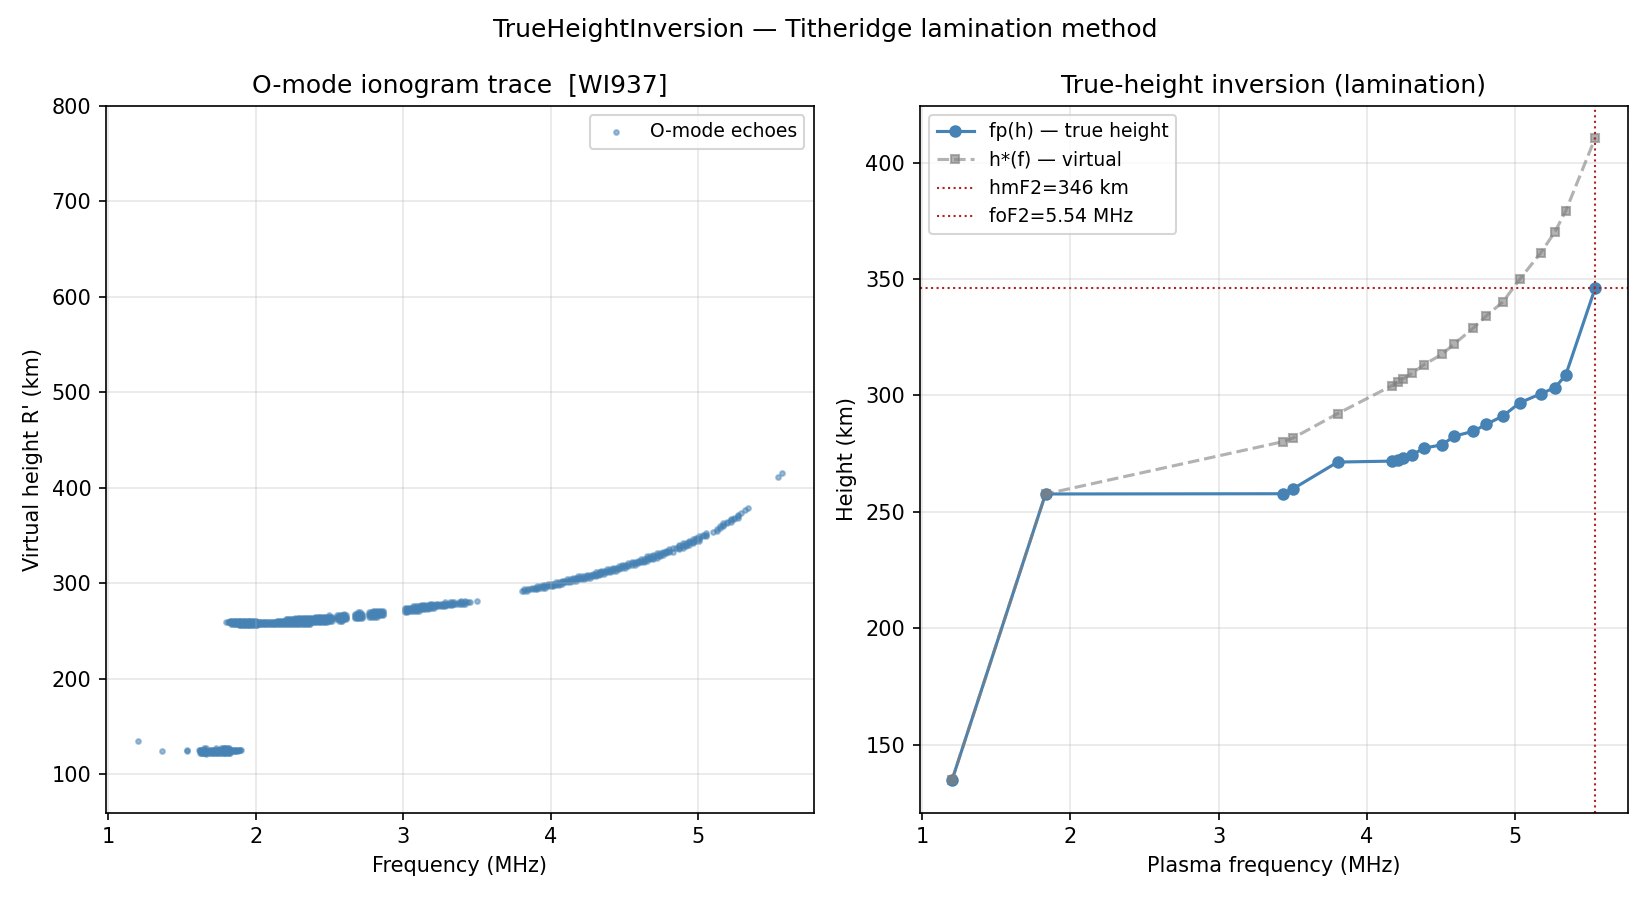
\includegraphics[width=0.90\linewidth]{analysis_inversion.png}
  \caption{True height inversion output: N(h) electron density profile
           (left) and virtual vs.\ true height comparison (right).}
  \label{fig:inversion}
\end{figure}

\begin{lstlisting}[caption={TrueHeightInversion API}]
from pynasonde.vipir.analysis import TrueHeightInversion
inv = TrueHeightInversion(monotone_enforce=True, bin_width_mhz=0.05)
edp = inv.fit_from_df(pol.annotated_df)  # O-mode filter applied automatically
print(edp.summary())   # foF2=8.12 MHz  hmF2=287.4 km  NmF2=8.2e5 cm^-3
\end{lstlisting}

%% ==================================================================
\section{Polarization \& Spread-F}
\label{sec:polar_spreadf}
%% ==================================================================

\begin{figure}[H]
  \centering
  \begin{minipage}{0.48\linewidth}
    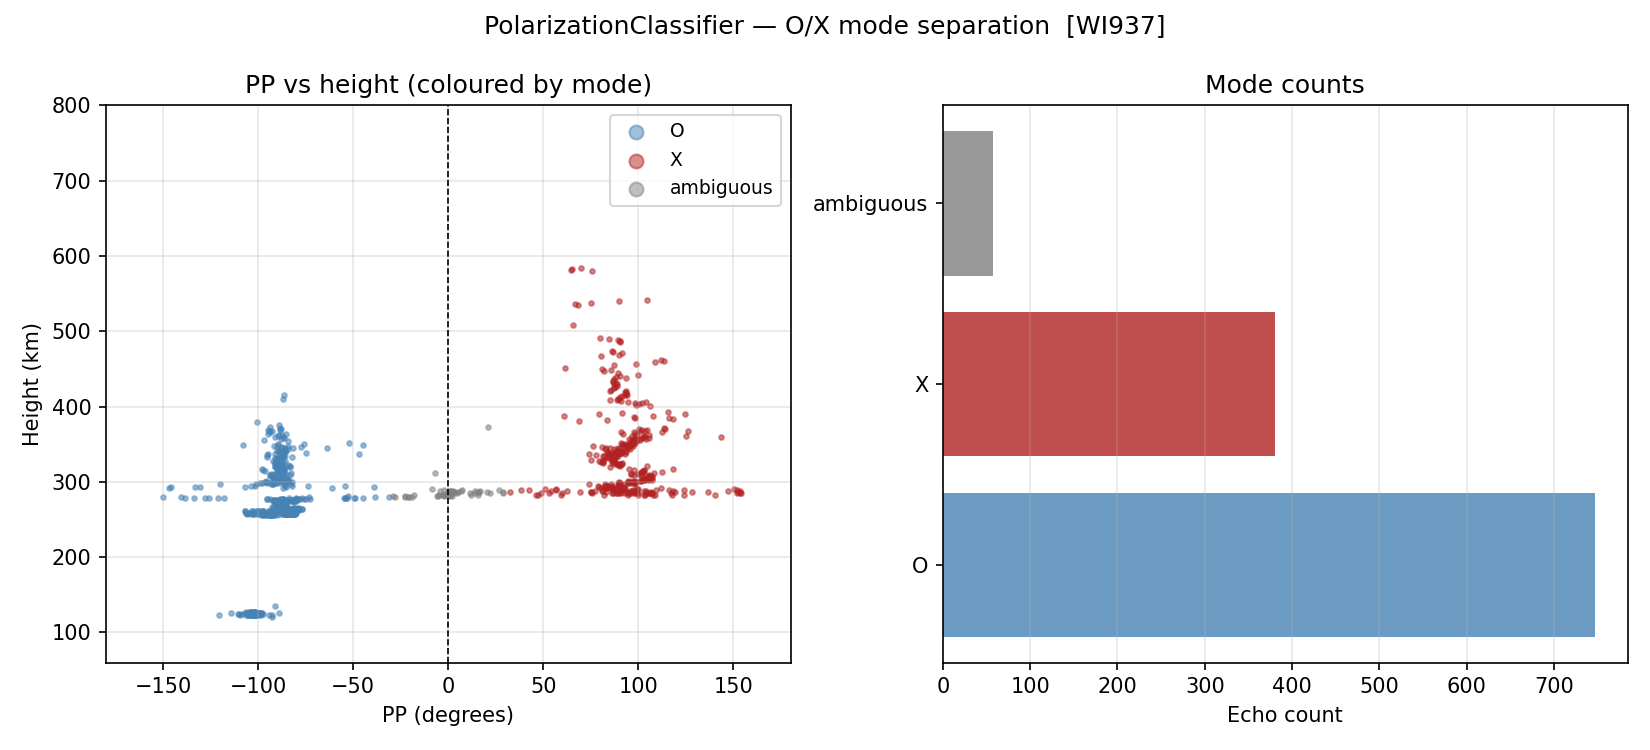
\includegraphics[width=\linewidth]{analysis_polarization.png}
    \caption{PP histogram with O/X classification regions.}
  \end{minipage}\hfill
  \begin{minipage}{0.48\linewidth}
    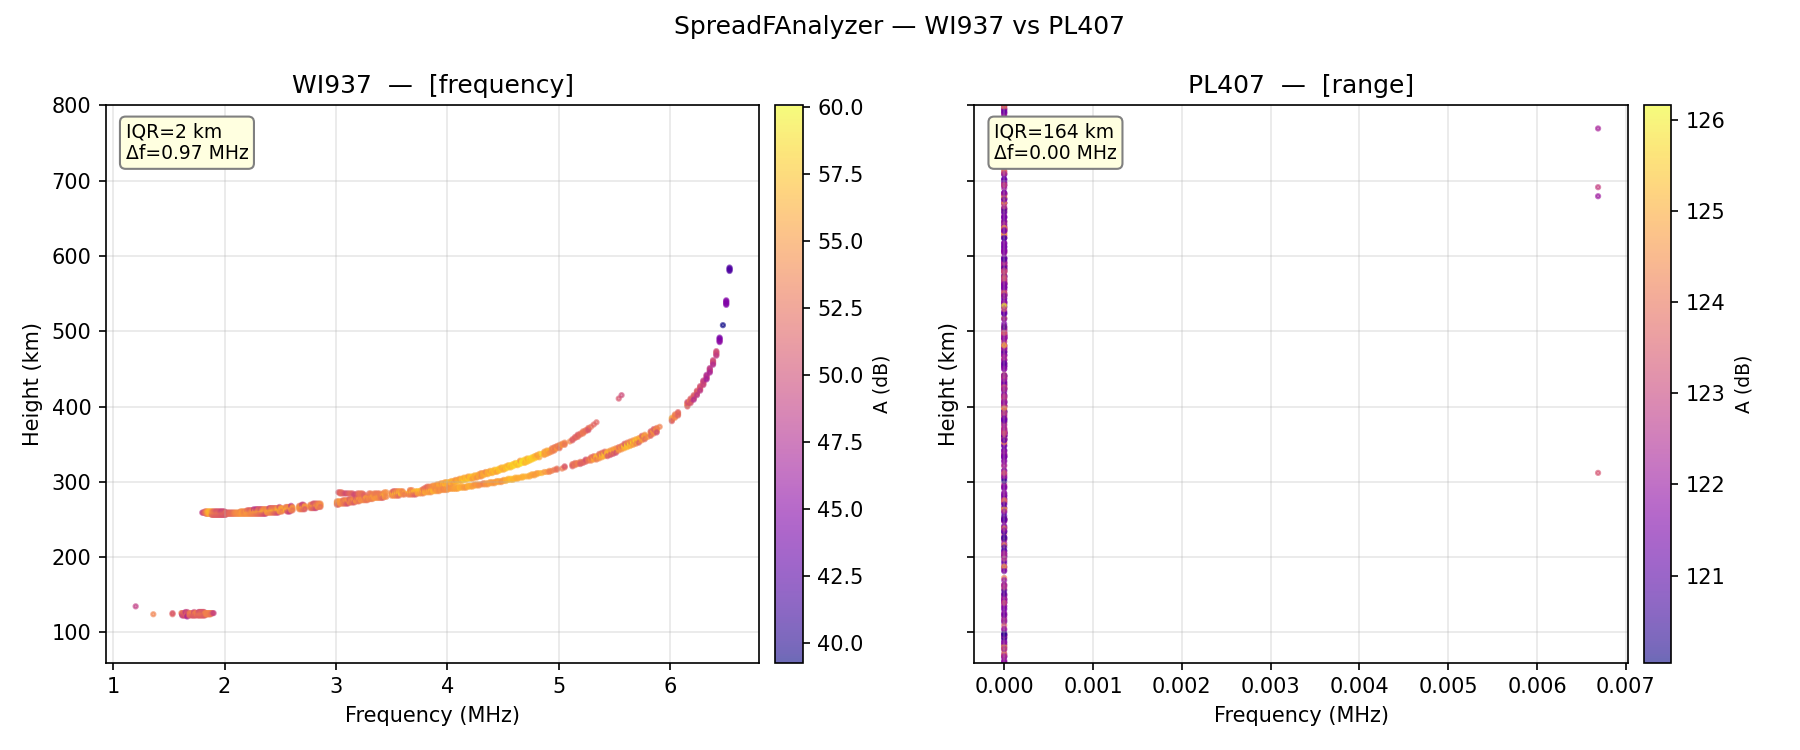
\includegraphics[width=\linewidth]{analysis_spread_f.png}
    \caption{Spread-F detection: range/frequency/mixed type classification.}
  \end{minipage}
\end{figure}

\begin{lstlisting}[caption={Polarization and Spread-F}]
from pynasonde.vipir.analysis import PolarizationClassifier, SpreadFAnalyzer

pol = PolarizationClassifier(o_mode_sign=-1).fit(filtered_df)
sf  = SpreadFAnalyzer().fit(filtered_df)
print(sf.summary())   # type=range  foEs=4.2 MHz  h_spread_km=38.1
\end{lstlisting}

%% ==================================================================
\section{Ionospheric Irregularity Analysis}
\label{sec:irregularities}
%% ==================================================================

\subsection{Physical motivation}

The EP (residual phase) parameter from the Dynasonde signal model carries
information about sub-wavelength irregularities in the ionospheric reflection layer.
Irregularities imprint a structured signature on EP as a function of sounding
frequency $f$.

\marginnotetext{EP is the wavefront residual phase: the part of the echo phase
not explained by the nominal group-range and Doppler shift.  Random phase
perturbations are evidence of small-scale density irregularities.}

\subsection{Structure function approach}

The second-order structure function of EP as a function of frequency lag $\Delta f$:
\begin{equation}
  D_{EP}(\Delta f) = \bigl\langle [EP(f+\Delta f) - EP(f)]^2 \bigr\rangle.
  \label{eq:strfunc}
\end{equation}
For a power-law irregularity spectrum with spectral index $\alpha$:
\begin{equation}
  D_{EP}(\Delta f) \propto \Delta f^\alpha.
  \label{eq:powerlaw}
\end{equation}
A log-log fit of $D_{EP}$ vs $\Delta f$ yields $\alpha$ and amplitude $A_0$.
The outer scale $L_{\mathrm{outer}}$ is estimated as the lag at which $D_{EP}$
saturates.

\subsection{Height-resolved and anisotropy analysis}

Echoes are binned by virtual height, and the fit is computed independently per bin,
giving a profile $\alpha(h)$.  When both O-mode and X-mode EP are available:
\begin{equation}
  \text{anisotropy proxy} = \frac{\sigma_{EP}(O)}{\sigma_{EP}(X)}.
  \label{eq:aniso}
\end{equation}
A ratio near unity indicates isotropic scattering; deviations indicate field-aligned anisotropy.

\begin{lstlisting}[caption={IrregularityAnalyzer API}]
from pynasonde.vipir.analysis import IrregularityAnalyzer

irr = IrregularityAnalyzer(
    height_bin_km=10.0,      # virtual height bin width
    min_echoes_per_bin=5,    # minimum echoes for a valid fit
    lag_max=2.0,             # maximum frequency lag (MHz) for structure function
)
result = irr.fit(filtered_df)
# result.profile_df: columns = height_km, alpha, A0, outer_scale_km, anisotropy
# result.alpha_profile:   1-D alpha(h) array
# result.outer_scale_km:  1-D L_outer(h) array
result.plot_spectral_profile()   # alpha(h) + outer scale overlay
result.plot_structure_function(height_km=200.0)  # D_EP vs lag at one height
\end{lstlisting}

%% ==================================================================
\section{NeXtYZ 3-D Electron Density Inversion}
\label{sec:nextyz}
%% ==================================================================

\subsection{Wedge-Stratified Ionosphere model}

The NeXtYZ algorithm (Zabotin et al.\ 2006) represents the local electron density
as a stack of plasma-frequency wedges bounded above by \emph{frame planes}.  Each
wedge boundary is characterised by:
\begin{equation}
  (h_{i+1},\; n_{x,i+1},\; n_{y,i+1}),
  \label{eq:wedge}
\end{equation}
where $h_{i+1}$ is the reflection height and $(n_x, n_y)$ are the horizontal
components of the outward normal — i.e., the ionospheric tilt.

\marginnotetext{NeXtYZ Lite solves only $h_{i+1}$ per wedge using constant tilts
derived from mean angles of arrival.  It is $\approx 6\times$ faster than Full mode
and sufficient for moderate tilt events.}

\subsection{Hamiltonian eikonal ray tracing}

Signal propagation through the WSI model is computed via the eikonal (method of
characteristics) equations:
\begin{align}
  \dot{\mathbf{r}} &= \partial H / \partial \mathbf{k}, \\
  \dot{\mathbf{k}} &= -\partial H / \partial \mathbf{r},
\end{align}
with Hamiltonian $H = |\mathbf{k}|^2 - n^2(\mathbf{r},f)$ and the full
Appleton-Lassen refractive index $n$.

\subsection{Inversion loop}

Wedge parameters are solved bottom-up by alternately minimising:
\begin{enumerate}
  \item \textbf{Group-range residual}:
    $\Delta R'_{i+1} = \sqrt{\sum_j (\rho'_{i+1,j} - R'_{i+1,j})^2}$
  \item \textbf{Ground-return distance} of the mean-direction ray (tilt constraint).
\end{enumerate}

\begin{lstlisting}[caption={NeXtYZInverter API}]
from pynasonde.vipir.analysis import NeXtYZInverter, NeXtYZResult

inv3d = NeXtYZInverter(
    mode="lite",          # "lite" (fast, const tilts) or "full" (per-wedge tilts)
    n_wedge_max=30,       # maximum number of WSI wedge layers
    ray_step_km=0.5,      # Hamiltonian integrator step size
    tilt_regularisation=0.01,  # weight of tilt constraint vs group-range fit
)
result: NeXtYZResult = inv3d.fit(filtered_df)

# Key output attributes
print(result.fp_profile)    # plasma frequency vs true height
print(result.tilt_x)        # E-W tilt per wedge (degrees)
print(result.tilt_y)        # N-S tilt per wedge (degrees)
print(result.height_error_km)  # estimated layer height uncertainty

result.plot_wedge_planes()  # 3-D visualisation of WSI frame planes
result.plot_fp_profile()    # fp(h) vs true height
\end{lstlisting}

%% ==================================================================
\section{API Quick-Reference}
\label{sec:api}
%% ==================================================================

\subsection{All public imports}

\begin{lstlisting}
# DIGISONDE I/O
from pynasonde.digisonde.parsers.sao import SaoExtractor, SaoSummaryPlots
from pynasonde.digisonde.parsers.rsf import RsfExtractor
from pynasonde.digisonde.parsers.sbf import SbfExtractor
from pynasonde.digisonde.parsers.dft import DftExtractor
from pynasonde.digisonde.parsers.dvl import DvlExtractor
from pynasonde.digisonde.parsers.sky import SkyExtractor, SkySummaryPlots
from pynasonde.digisonde.parsers.edp import EdpExtractor

# VIPIR I/O
from pynasonde.vipir.riq.parsers.read_riq import RiqDataset, VIPIR_VERSION_MAP
from pynasonde.vipir.riq.echo import EchoExtractor
from pynasonde.vipir.riq.parsers.filter import IonogramFilter
from pynasonde.vipir.ngi.source import DataSource
from pynasonde.vipir.ngi.scale import AutoScaler

# Analysis layer
from pynasonde.vipir.analysis import (
    PolarizationClassifier, PolarizationResult,
    TrueHeightInversion, EDPResult,
    AbsorptionAnalyzer, LOFResult, DifferentialResult,
    TotalAbsorptionResult, AbsorptionProfileResult,
    SpreadFAnalyzer, SpreadFResult,
    IrregularityAnalyzer, IrregularityProfile,
    IonogramScaler, ScaledParameters,
    EsCaponImager, RiqAggregator, EsImagingResult,
    NeXtYZInverter, NeXtYZResult, WedgePlane,
)
\end{lstlisting}

\subsection{Constructor summary}

\begin{table}[H]
  \centering
  \caption{Key constructor parameters for all analysis classes.}
  \small
  \begin{tabular}{llll}
    \toprule
    Class & Parameter & Default & Notes \\
    \midrule
    \multirow{4}{*}{\texttt{EsCaponImager}}
      & \texttt{n\_subbands}        & 100     & $Z$; recommended $\le (V{+}1)/2$ \\
      & \texttt{resolution\_factor} & 10      & $K$; no singularity limit \\
      & \texttt{gate\_spacing\_km}  & 3.84    & $r_0$; VIPIR WI937 = 1.499 km \\
      & \texttt{diagonal\_loading}  & 1e-3    & $\varepsilon$ for $\Rf$ conditioning \\
    \midrule
    \multirow{3}{*}{\texttt{RiqAggregator}}
      & \texttt{rx\_weights}        & None    & None = uniform $1/n_{rx}$ \\
      & \texttt{output\_mode}       & single  & or \texttt{slow\_rti} \\
      & \texttt{gate\_spacing\_km}  & 1.499   & overridden from RIQ header \\
    \midrule
    \multirow{3}{*}{\texttt{TrueHeightInversion}}
      & \texttt{method}             & lamination & only supported method \\
      & \texttt{bin\_width\_mhz}    & 0.05    & trace decimation for stability \\
      & \texttt{monotone\_enforce}  & True    & remove non-monotone layers \\
    \midrule
    \texttt{AbsorptionAnalyzer}
      & \texttt{f\_ref\_mhz}        & 1.0     & quiet-day reference for LOF \\
    \midrule
    \texttt{PolarizationClassifier}
      & \texttt{o\_mode\_sign}      & $-1$    & $+1$ for southern hemisphere \\
    \midrule
    \multirow{3}{*}{\texttt{IrregularityAnalyzer}}
      & \texttt{height\_bin\_km}    & 10.0    & virtual height bin width \\
      & \texttt{min\_echoes\_per\_bin} & 5   & minimum for valid power-law fit \\
      & \texttt{lag\_max}           & 2.0~MHz & max frequency lag for $D_{EP}$ \\
    \midrule
    \multirow{4}{*}{\texttt{NeXtYZInverter}}
      & \texttt{mode}               & \texttt{lite}  & \texttt{lite} (fast) or \texttt{full} (per-wedge tilts) \\
      & \texttt{n\_wedge\_max}      & 30      & maximum WSI wedge layers \\
      & \texttt{ray\_step\_km}      & 0.5     & Hamiltonian integrator step size \\
      & \texttt{tilt\_regularisation} & 0.01 & tilt constraint weight \\
    \bottomrule
  \end{tabular}
\end{table}

\subsection{Result dataclasses at a glance}

\begin{table}[H]
  \centering
  \caption{Key attributes of result objects.}
  \small
  \begin{tabular}{lll}
    \toprule
    Class & Key attributes & Shape \\
    \midrule
    \texttt{EsImagingResult}
      & \texttt{pseudospectrum\_db} & $(n_s, KV)$ \\
      & \texttt{heights\_km}       & $(KV,)$ \\
      & \texttt{effective\_resolution\_km} & scalar \\
    \midrule
    \texttt{EDPResult}
      & \texttt{true\_height\_km}, \texttt{plasma\_freq\_mhz} & $(n_L,)$ \\
      & \texttt{foF2\_mhz}, \texttt{hmF2\_km}, \texttt{NmF2\_cm3} & scalar \\
    \midrule
    \texttt{AbsorptionProfileResult}
      & \texttt{profile\_df} ($h$, $\nu$, $f_p$, $X$, $\kappa$) & DataFrame \\
      & \texttt{total\_absorption\_db} & scalar \\
    \midrule
    \texttt{PolarizationResult}
      & \texttt{annotated\_df} (\texttt{mode} column) & DataFrame \\
      & \texttt{o\_mode\_count}, \texttt{x\_mode\_count} & int \\
    \bottomrule
  \end{tabular}
\end{table}

%% ==================================================================
\section*{References}
%% ==================================================================

\begin{itemize}\small
  \item Liu, T., Yang, G., \& Jiang, C. (2023). High-resolution sporadic E layer
        observation. \textit{Space Weather}, 21, e2022SW003195.
        \url{https://doi.org/10.1029/2022SW003195}
  \item Titheridge, J.\ E. (1967). \textit{JATP}, 29, 763--778.
  \item Paul, A.\ K. (1975). POLAN. \textit{NOAA Technical Report ERL 324-SEL 31}.
  \item Zabotin, N.\ A., Wright, J.\ W., \& Zhbankov, G.\ A. (2006). NeXtYZ.
        \textit{Radio Science}, 41, RS6S32.
  \item Davies, K. (1990). \textit{Ionospheric Radio}. Peter Peregrinus.
  \item Budden, K.\ G. (1985). \textit{The Propagation of Radio Waves}. Cambridge.
  \item Grubb, R.\ N., et al.\ (2011). New science with VIPIR. \textit{Radio Science}.
  \item Reinisch, B.\ W., et al.\ (1997). The Digisonde 4D. \textit{JASTP}, 59, 2181.
\end{itemize}

\end{document}
